\documentclass{article}
\usepackage[utf8]{inputenc}
\usepackage[a4paper, total={6in, 8in}, margin = 3cm]{geometry}
\usepackage[english]{babel}
\usepackage{authblk}
\usepackage{enumitem}
\usepackage{mathtools}
\usepackage{amssymb}
\usepackage{amsmath}
\usepackage{setspace}
\usepackage{natbib}
\usepackage{subfigure}
\usepackage{todonotes} % for comments


\newcommand{\ziang}{\textcolor{blue}}


\title{\textbf{Bayesian smoothing with extended second order random walk model: An detailed overview and comparison}}

\author{
Ziang Zhang \\ \vspace{-0.3cm}\normalsize\texttt{aguero.zhang@mail.utoronto.ca}\\ 
\large
\vspace{0.5cm}
Supervisor(s): James Stafford, Patrick Brown \\ 

\vspace{0.5cm}
Department of Statistical Sciences \\
University of Toronto
}

\date{June 2021}

\onehalfspacing


\begin{document}


\maketitle


\newpage

\begin{abstract}
In this report, we will describe and implement the extended second order random walk model proposed in \cite{rw2}. This method can be viewed as an extension of the formerly used second order random walk model to irregular spaced locations, derived from discretizing a stochastic differential equation. We will compare this method with other Bayesian smoothing spline methods, both conceptually and practically. This report will provide practitioners with a more thorough understanding of the connection between the second order random walk model and other Bayesian smoothing methods, and a practical guideline on how to choose among these methods.
\end{abstract}


\bigskip

\tableofcontents

\newpage


\section{Introduction}\label{intro}

Smoothing methods are often used when there is little information on the functional structures of some covariate effects. The main challenging of smoothing is to provide enough flexibility so that the functional form of covariate effect can be accurately inferred without over-fitting the observed data. In smoothing spline method, this trade off is controlled by a smoothing parameter $\lambda$, which penalizes the wiggliness of inferred function. 

Consider a data set $\{y_i,x_i, i\in [n]\}$, and a nonparametric model $y_i = g(x_i) + \epsilon_i$ where $\epsilon_i \overset{iid}\sim N(0,\sigma_\epsilon^2)$ and $x_i \in [a,b]$, then the smoothing spline aims to solve the following problem:
\begin{equation}\label{equ:ss}
\arg\min_{g\in C^2} \bigg\{ \sum_i\bigg(y_i-g(x_i)\bigg)^2 + \lambda \sigma_\epsilon^2 \int_a^b g''(x)^2 dx \bigg\}
\end{equation}
The sum of square term on the left can be replaced by negative log likelihood, which is also called \textit{penalized likelihood} method.

In typical frequentist method, the smoothing parameter $\lambda$ is either taken as fixed value input by the users, or substituted by an optimal value selected from procedure such as REML. Therefore, how to take into account the uncertainty with the unknown hyper-parameter increases the difficulty of frequentist smoothing methods. On the other hand, the hyper-parameter $\lambda$ will be assigned with a prior distribution in Bayesian smoothing methods, and hence any uncertainty involved with that parameter will be taken into account for the inference. Furthermore, the development of approximate Bayesian inference methods such as \cite{inla} enables Bayesian smoothing to be implemented in a computationally convenient way. Because of the ability to yield model-based estimation and uncertainty quantification for all parameters of interest, application of Bayesian smoothing method can be advantageous in a lot of settings.


Based on the well known connection between smoothing splines and integrated Wiener processes \citep{wahba}, \cite{rw2} developed a Bayesian smoothing method by assigning a stochastic differential equation (SDE) based prior to the unknown true effect functions. 
Their method uses a finite element method called Galerkin approximation to the SDE, and then solves for its weak solution. Therefore, the method of \cite{inla} can be viewed as an extension of the second order random walk model (RW2) to irregular spaced locations.
The hyper-parameter $\sigma_s$ which is defined as $\sigma_s^2 = \frac{1}{ \lambda \sigma_\epsilon^2}$, represents the standard deviation parameter of the second derivative of the covariate effect function, and will be assigned with a proper prior distribution. Because of the use of numerical approximation, the resulting prior distribution for the effect function will have a sparse precision matrix, and hence will be computationally efficient if used together with approximate Bayesian inference method such as Integrated Nested Laplace Approximation (INLA) \citep{inla}. Both theoretical results and simulation results have been demonstrated for their Galerkin approximation methods in their original paper \citep{rw2}.


In section \ref{SmoothSpline}, we will describe how is smoothing spline typically fitted in Frequentist method, and how it can be reinterpreted as an equivalent Bayesian inference problem with ARIMA prior when locations are equally spaced \citep{ARIMA}. In section \ref{rw2}, we will introduce the extended second order random walk method proposed in \cite{rw2}, and provide conceptual comparison and connection with the the exact method using ARIMA method. Furthermore, we will write the ARIMA method in the form of a similar SDE specification, and hence generalize the ARIMA method to irregular spaced locations and enhances its computational efficiency. In section \ref{practice}, we will implement several simulation studies to illustrate the differences between all the mentioned Bayesian smoothing spline methods, in aspects of inferences for both the function and its higher order derivatives. We conclude in section \ref{conclusion} with a discussion.


\section{Smoothing Spline}\label{SmoothSpline}

\subsection{Fitting Smoothing Spline}

Consider the smoothing parameter $\lambda$ in equation \ref{equ:ss} is a fixed constant, the solution to the \textit{penalized likelihood} equation \ref{equ:ss}, denoted as $\hat{g}_\lambda(.)$, is well known to be a natural cubic polynomial spline when the response variable $\boldsymbol{y}:= (y_1, y_2, ..., y_n)^T \in \mathbb{R}^n$ cannot be perfectly interpolated by a lower order polynomial function. For any function $g$, let $\boldsymbol{g} := (g(x_1), ..., g(x_n))^T \in \mathbb{R}^n$ denotes the corresponding evaluation vector, then the solution cubic spline $\hat{g}_\lambda(.)$ can be uniquely determined based on its evaluation vector $\boldsymbol{\hat{g}_\lambda}$ \citep{smoothingspline}. 



Using the property of natural cubic spline, the term $\int_a^b g''(x)^2 dx$ for any natural cubic spline $g(.)$ can be written as $\boldsymbol{g}^T K \boldsymbol{g}$, where the matrix $K$ only depends on the covariate locations $\boldsymbol{x} := (x_1, ..., x_n)^T \in \mathbb{R}^n$, not on the response variable $\boldsymbol{y}$. Therefore, the equation \ref{equ:ss} in section \ref{intro} can be written in the following vector form:
\begin{equation}\label{equ:vectorss}
\arg\min_{\boldsymbol{g}\in \mathbb{R}^n} \frac{1}{ \sigma_\epsilon^2}(\boldsymbol{y} - \boldsymbol{g})^T (\boldsymbol{y} - \boldsymbol{g}) + \lambda \boldsymbol{g}^T K \boldsymbol{g}.
\end{equation}
Since this function is convex in $\boldsymbol{g}$, taking derivative and setting it to zero yields the evaluation vector $\boldsymbol{\hat{g}_\lambda} = (I+\lambda \sigma_\epsilon^2 K)^{-1} \boldsymbol{y}$. Hence the solution function can be recovered from this evaluation vector. 

The above procedures all treat the single smoothing parameter $\lambda$ as a fixed constant. In practice, there are two common ways to select the value of $\lambda$: selecting a constant based on the subjective belief on the required smoothness of the fitted function or estimating its value based on the observed data \citep{smoothingspline}. 

If one decides to estimate the smoothing parameter using the same set of data, methods such as cross-validation (CV), generalized cross-validation(GCV) or restricted maximum likelihood estimation (REML) can be used. When computing quantities such as confidence intervals and standard errors, traditional frequentist approaches will directly plug in the estimate of $\lambda$ and treat it as a known value. Therefore the traditional frequentist inference methods will tend to underestimate the variability, because they ignore the additional uncertainty from the estimation of $\lambda$. For this reason, Bayesian smoothing methods which fully take into account the uncertainty with the value of $\lambda$ can be preferred at many applications.










\subsection{Bayesian Smoothing Spline with ARIMA Model}\label{ARIMA}

Besides the frequentist penalized likelihood interpretation, the smoothing spline can also be interpreted as a Bayesian inference problem with partially diffuse priors \citep{ARIMA}. For simplicity, we will assume the variance parameter $\sigma_\epsilon = 1$ is fixed.
Recall in the vectorized (negative) penalized likelihood equation \ref{equ:vectorss}, the first term can be regarded as the (negative) log likelihood $\log f(\boldsymbol{y}|\boldsymbol{g},\lambda)$, and the second term can be viewed as the (negative) log prior for $\boldsymbol{g}$, denoted as $\log f(\boldsymbol{g})$. If we also assume the smoothing parameter $\lambda$ is a known constant, then equation \ref{equ:vectorss} can be interpreted as (negative) log joint likelihood $\log f(\boldsymbol{y},\boldsymbol{g})$ which has the same maximum $\hat{\boldsymbol{g}}$ as the log posterior $\log f(\boldsymbol{g}|\boldsymbol{y})$.

The likelihood above corresponds to $\boldsymbol{y}|\boldsymbol{g} \sim N(0, I)$, and the prior for $\boldsymbol{g}$ corresponds to $\boldsymbol{g} \sim N(0, \frac{1}{\lambda} K^{-1})$. The assumption that $\sigma_\epsilon = 1$ here is not stringent, as one can reparametrize the parameter $\lambda$ as $\lambda\sigma_\epsilon^2$ without changing the shape of the posterior for $\boldsymbol{g}$.
To better understand the prior for $\boldsymbol{g}$, note that the precision matrix $K$ can be factorized as the following:
\begin{equation}\label{equ:ArimaPrior}
K = D^T R^{-1} D.
\end{equation}
When all the locations are equally spaced with unit spacings, the $(n-2) \times n$ matrix $D$ will be the second order difference matrix defined as:
\begin{equation}
\begin{aligned}
D = \mbox{\scriptsize $\begin{bmatrix}
1 & -2 & 1 & 0 & 0 & \cdots & 0\\
0 & 1 & -2 & 1 & \cdots & 0 & 0\\
0 & \vdots &  &  & \ddots & 0 & 0\\
0 & 0 & 0 & \cdots & 1 & -2 & 1\\
\end{bmatrix}$}
\end{aligned},
\end{equation}

and the $(n-2) \times (n-2)$ matrix R is a strictly positive definite matrix that can be computed as:
\begin{equation}
\begin{aligned}
R = \mbox{\scriptsize $\begin{bmatrix}
\frac{2}{3} & \frac{1}{6} & 0 & 0 & 0 & \cdots & 0\\
\frac{1}{6} & \frac{2}{3} & \frac{1}{6} & 0 & 0 & \cdots & 0\\
0 & \frac{1}{6} & \frac{2}{3} & \frac{1}{6} & 0 & \cdots & 0\\
 &  &  &  &  & \ddots & \\
0 & 0 & 0 & \cdots & 0 & \frac{1}{6} & \frac{2}{3}\\
\end{bmatrix}$}
\end{aligned}.
\end{equation}

Note that the $D$ matrix can be viewed as a second order difference operator, that functions on the evaluation vector $\textbf{g}$ to get its second order difference vector $\boldsymbol \gamma := D \boldsymbol g$. Hence $\boldsymbol g^TK \boldsymbol g$ can be equivalently computed as $\boldsymbol \gamma^T R^{-1} \boldsymbol \gamma$. In other words, if we define $\sigma_s^2 := \frac{1}{\lambda}$, adding the penalty term is equivalent to assigning a prior to the second order difference vector $\boldsymbol \gamma \sim N(0,\sigma_s^2R)$.

Let $\boldsymbol \gamma:=(\gamma_3,...,\gamma_n)^T \in \mathbb{R}^{n-2}$, with $\gamma_i :=g(x_i)-2g(x_{i-1})+g(x_{i-2})$, then we can notice that the covariance matrix $R$ of $\boldsymbol \gamma$ has the same structure as a MA(1) model. Let $\boldsymbol \xi :=(\xi_2,...,\xi_n)^T \sim N(0, I)$, and define $\gamma_i = \theta\xi_{i-1} +\xi_i$, then we can write $\boldsymbol \gamma = \Theta \boldsymbol \xi$, where the $(n-2)\times(n-1)$ coefficient matrix $\Theta$ is defined as:
\begin{equation}
\begin{aligned}
\Theta = \mbox{\scriptsize $\begin{bmatrix}
\theta & 1 & 0 & 0 & 0 & \cdots & 0\\
0 & \theta & 1 & 0 & 0 & \cdots & 0\\
0 & 0 & \theta & 1 & 0 & \cdots & 0\\
 &  &  &  &  & \ddots & \\
0 & 0 & 0 & \cdots & 0 & \theta & 1\\
\end{bmatrix}$}
\end{aligned}.
\end{equation}

To solve the coefficient $\theta$, we want to find the value such that $\Theta\Theta^T=R$. This gives $\theta = 2 \pm \sqrt{3}$, and we will select $\theta=2-\sqrt3 <1$ so that the process is invertible. Putting such MA(1) prior on the second order difference vector implies an ARIMA(0,2,1) prior will be assigned to the parameter vector $\boldsymbol g$ \citep{ARIMA}.

With this Bayesian interpretation of the smoothing spline problem, the frequentist maximum penalized likelihood estimate $\boldsymbol{\hat{g}_\lambda}$ can also be viewed as the posterior mode when an ARIMA prior is assigned to $\boldsymbol g$. Furthermore, when the likelihood is Gaussian as above, it will also be the posterior mean, since the posterior of $\boldsymbol g$ is also Gaussian in this case.

Besides providing an another interpretation for the smoothing spline problem, this Bayesian setting also provides easy ways to account for the uncertainty with respect to the smoothing parameter $\lambda$, by assigning a prior for it and considering a Bayesian hierarchical model. 

This Bayesian smoothing spline interpretation with ARIMA prior will only be valid when all the locations are equally spaced. If locations are not equally spaced, one can consider cutting the locations into a finer grid to achieve equal spacing. This amounts to create a larger dataset with a lot of missing values for the response variable $y$, but this augmented dataset will only be used to construct the covariance matrix for $\boldsymbol{\gamma}$ and hence these missing $y$ will not become a problem in the computation of $\hat{\boldsymbol{g}}$.




\section{Extended Second Order Random Walk Method To Smoothing Spline}\label{rw2}

\subsection{Prior Based On Stochastic Differential Equation}\label{SDEprior}


Although the ARIMA approach in \cite{ARIMA} provides a very useful Bayesian interpretation of the \textit{exact} smoothing spline problem, this approach may encounter the following two problems.
First, the precision matrix $K$ of the ARIMA prior is dense, and it has dimension growing with the sample size $n$. When sample size is very large, Bayesian inference for such model becomes too computationally demanding to achieve.
Furthermore, although the data augmentation tricks can generalize the use of such ARIMA prior to irregular spaced locations, it further increases the dimension of the dense precision matrix $K$, and hence compounds the computational burden.

An alternative method is to assign a prior on the whole unknown function $g(.)$, instead of its evaluation vector $\boldsymbol g :=(g(x_1),..,g(x_n))^T$. This can be done through the use of stochastic differential equation (SDE) based prior on the function space. Let $W(t)$ denote the standard Wiener's process (Brownian motion), a SDE based prior is assigned to $g(t)$ in the following way:
$$\frac{d^2g(t)}{dt^2} = \sigma_s\frac{dW(t)}{dt}.$$ 
The derivative of $W(t)$ does not exist in ordinary definition, but can be defined as a generalized function, the \textit{white noise} process. Such SDE will not be well defined without extra conditions on the intercept $g(0)$ and the 
slope $g'(0)$. When $g(0)$ and $g'(0)$ are fixed to be zero, this SDE is equivalent to use a \textit{second folded Wiener's process} on $g(t)$. In the case of Gaussian likelihood, if $g(0)$ and $g'(0)$ are given diffuse Gaussian priors, the limiting posterior mean of $\boldsymbol g$ will be the minimizer of the smoothing spline problem \citep{wahba}.


\subsection{Finite Element Method and Weak Solution}

The direct use of such SDE prior on $g(x)$ can yield posteriors for the evaluation vector $\boldsymbol g$, but the posterior of $g(s)$ for $s \notin \{x_i,i\in[n]\}$ cannot be directly obtained from $P(\boldsymbol g|y)$. To reduce the problem of inference for infinite dimension parameter $g(.)$ to finite dimensional inference, it is convenient to consider the use of \textit{Finite Element Method} to discretize the SDE.

The Finite Element Method can be understood as the following procedures. Let $\mathbb{B}_p:=\{\varphi_i, i \in [p] \}$ denote the set of $p$ pre-specified basis functions, and let $\mathbb{T}_q:=\{\phi_i, i \in [q]\}$ denote the set of $q$ pre-specified test functions. We consider an finite dimensional approximation $\tilde{g}(.)$ to the true function $g(.)$, defined as:
\begin{equation}\label{discretization}
\tilde{g}(.) = \sum_{i=1}^{p}w_i \varphi_i(.),
\end{equation}
where $\boldsymbol{w} := (w_1,...,w_p)^T \in \mathbb{R}^p$ is a set of weights that is to be determined. 

To determine the unknown weight vector $\boldsymbol{w}$, we seek the weak solution of the SDE relative to the test functions $\mathbb{T}_q$, that is:
\begin{equation}\label{weakSol}
\langle \frac{d^2\tilde{g}(t)}{dt^2} , \phi_i(t)\rangle \overset{d}= \langle \sigma_s\frac{dW(t)}{dt} , \phi_i(t)\rangle,
\end{equation}
for any test function $\phi_i \in \mathbb{T}_q$. This equation \ref{weakSol} implicitly defines the prior distribution on the finite dimensional weight vector, which will be multivariate Gaussian with precision matrix structure depending on the choice of $\mathbb{T}_q$ and $\mathbb{B}_p$. Specifically, the inner products $\langle \frac{d^2\tilde{g}(t)}{dt^2} , \phi_i(t)\rangle_{i=1}^q$ can be vectorized as $$\langle \frac{d^2\tilde{g}(t)}{dt^2} , \phi_i(t)\rangle_{i=1}^q =H \boldsymbol w,$$ where the $ij$ component of the $q \times p$ $H$ matrix can be computed as $$H_{ij} = \langle \frac{d^2\phi_j(t)}{dt^2} , \phi_i(t)\rangle_{i=1}^q.$$

The second inner products $\langle \frac{dW(t)}{dt} , \phi_i(t)\rangle_{i=1}^q$ will have Gaussian distribution with zero mean vector and $q \times q$ covariance matrix $B_{ij}=[\langle \phi_i ,\phi_j\rangle]$.

There are two different types of Finite Element Method, called \textit{Bubnov Galerkin} and \textit{Petrov Galerkin}. If the set of basis function $\mathbb{B}_p$ and the set of test function $\mathbb{T}_q$ are the same, the Finite Element Method is called Bubnov-Galerkin approximation. Otherwise the Finite Element Method is called Petrov-Galerkin approximation.




\subsection{The Extended Second Order Random Walk Method}

In \cite{rw2}, the authors proposed an extension of the commonly used Second Order Random Walk Method (RW2) to irregular spaced locations. When $\boldsymbol{x}$ has equal spacings, the original RW2 model specifies a joint density to $\boldsymbol{g}$ as the following:
\begin{equation}\label{oldrw2}
f(\boldsymbol{g}) = \frac{1}{\sigma_s^{(n-2)}} \exp \bigg( -\frac{1}{2 \sigma_s^2} \sum_{i=1}^{n-2} (g(x_i) - 2g(x_{i+1}) + g(x_{i+2}))^2 \bigg).
\end{equation}
This type of model is called second order \textit{Intrinsic Gaussian Markov random fields} (IGMRF), because it is invariant to the addition of polynomials with order less than two \citep{rue2005gaussian}. The RW2 model is computationally efficient to be used in approximate Bayesian inference method, since it can be rewritten as the following:
\begin{equation}\label{alter-oldrw2}
f(\boldsymbol{g}) = \frac{1}{\sigma_s^{(n-2)}} \exp \bigg( -\frac{1}{2} \boldsymbol{g}^T Q \boldsymbol{g}  \bigg),
\end{equation}
where the precision matrix $Q$ is a sparse matrix defined as:

\begin{equation}
\begin{aligned}
Q = \mbox{\scriptsize $ \frac{1}{\sigma_s^2} \begin{bmatrix}
1 & -2 & 1 &  &  &  & &  & & \\
-2 & 5 & -4 & 1 &  &  & &  & & \\
1 & -4 & 6  & -4 & 1 &  & &  & & \\
 & 1 & -4 & 6  & -4  & 1  & &  & & \\
 &  & 1 & -4 & 6  & -4  & 1  & & & \\
 & &  & & & & & & & \\
  & &  & & & \ddots & \ddots & \ddots & & \\
   &  &  &  &   &   &  1 &-2 & 1 & \\
\end{bmatrix}
$}
\end{aligned}.
\end{equation}

The sparsity of this precision matrix comes from the conditional independence structure of $\boldsymbol{g}$, and can be efficiently utilized by inference method such as integrated nested laplace approximation (INLA) \citep{inla}. When locations are not equally spaced, one can consider ad-hoc method such as refining the resolution to finer, equally spaced locations. However, as mentioned in \cite{rue2005gaussian}, this RW2 model will not be consistent with different resolutions for the grid.

To find a consistent extension of the RW2 model to irregular space, \citep{rw2} considered an alternative derivation derived from the continuous time stochastic process defined by the SDE in section \ref{SDEprior}. The authors proposed the use of Bubnov-Galerkin method to discretize the SDE into a finite dimensional problem, and use the set of $n$ linear B spline functions defined on the locations $\boldsymbol{x}$ as both the basis functions and the test functions. If we still assume unit-spaced locations for simplicity, the corresponding $H$ matrix and $B$ matrix can be respectively computed as:
\begin{equation}\label{HandB}
\begin{aligned}
H = \mbox{\scriptsize $\begin{bmatrix}
0 & 0 & 0 & 0 & 0 & \cdots & 0\\
1 & -2 & 1 & 0 & 0 & \cdots & 0\\
0 & 1 & -2 & 1 & \cdots & 0 & 0\\
0 & \vdots &  &  & \ddots & 0 & 0\\
0 & 0 & 0 & \cdots & 1 & -2 & 1\\
0 & 0 & 0 & 0 & 0 & \cdots & 0\\
\end{bmatrix}$},
B = \mbox{\scriptsize $\begin{bmatrix}
\frac{1}{3} & \frac{1}{6} & 0 & 0 & 0 & \cdots & 0 & 0\\
\frac{1}{6} & \frac{2}{3} & \frac{1}{6} & 0 & 0 & \cdots & 0 & 0\\
0 & \frac{1}{6} & \frac{2}{3} & \frac{1}{6} & 0 & \cdots & 0 & 0\\
0 & 0 & \frac{1}{6} & \frac{2}{3} & \frac{1}{6} & \cdots & 0 & 0\\
 &  &  &  & \ddots &  & & \\
 0 & 0 & 0 & \cdots & \frac{1}{6} & \frac{2}{3} & 0 & 0\\
0 & 0 & 0 & \cdots & 0 & \frac{1}{6} & \frac{2}{3} & 0\\
0 & 0 & 0 & \cdots & 0 & 0 & \frac{1}{6} & \frac{1}{3} \\
\end{bmatrix}$}.
\end{aligned}
\end{equation}
As noted in \cite{rw2}, this Galerkin \textit{approximation} is actually exact, except for the boundaries. This can also be found from the fact that $H$ matrix after removing its first and last row is the $D$ matrix from \cite{ARIMA}, and the $B$ matrix after removing its first and last rows and columns is the $R$ matrix from \cite{ARIMA}.

The use of Galerkin approximation as in \cite{rw2} will result in $\boldsymbol w$ having precision matrix $H^TB^{-1}H$. Since $B$ matrix is tri-diagonal, this precision matrix will be dense, and hence not applicable in INLA-typed inference method \citep{inla}. To handle this dense precision matrix problem, \cite{rw2} proposes the use of a diagonal approximation $A$, to the covariance matrix $B$. This diagonal approximation $A$ can be gotten by distributing the off-diagonal values in $B$ to its main diagonal, which has been shown in \citep{rw2} to have small long-term effect in the final precision matrix.

Specifically in the unit-spaced case above, the covariance matrix $B$ is approximated by the diagonal matrix A defined as following:
\begin{equation}
\begin{aligned}
A = \mbox{\scriptsize $\begin{bmatrix}
\frac{1}{2} & 0 & 0 & 0 & 0 & \cdots & 0 & 0\\
0 & 1 & 0 & 0 & 0 & \cdots & 0 & 0\\
0 & 0 & 1 & 0 & 0 & \cdots & 0 & 0\\
0 & 0 & 0 & 1 & 0 & \cdots & 0 & 0\\
 &  &  &  & \ddots &  & & \\
 0 & 0 & 0 & \cdots & 0 & 1 & 0 & 0\\
0 & 0 & 0 & \cdots & 0 & 0 & 1 & 0\\
0 & 0 & 0 & \cdots & 0 & 0 & 0 & \frac{1}{2} \\
\end{bmatrix}$}
\end{aligned}.
\end{equation}

This amounts to use uncorrelated noises to approximate the noises $\langle \frac{dW(t)}{dt} , \phi_i(t)\rangle_{i=1}^n$
which approximately have a MA(1) covariance structure. The resulting (approximate) Galerkin approximation is the extended second order random walk prior. Note that with this diagonal approximation, the extended RW2 model will always have a sparse precision matrix regardless of the spacings between locations. When the locations are equally spaced, the extended RW2 model then simplifies to the original RW2 model defined in equation \ref{alter-oldrw2}. As shown in \cite{rw2}, the covariance property of this approximation will converge to the original continuous process defined in the SDE, as the density of locations increases.

It is worth notice that when locations are equally spaced, the exact Bayesian representation of the smoothing spline problem using ARIMA model can also be rewritten using the same SDE-discretization method above. If we keep the same set of linear spline functions to be the $n$ basis functions, but remove $\phi_1$ and $\phi_n$ from the set of test functions, then the same discretization procedure will yield $D^TR^{-1}D$ as the precision matrix, the same precision matrix of the ARIMA model. In other words, this \textit{Petrov Galerkin} procedure will have a weak solution that is also the exact solution to the SDE, even at the boundaries.

This SDE representation of the ARIMA method will have the following two implications. First, this ARIMA-based Bayesian interpretation of smoothing spline can be generalized to the case where locations are irregularly spaced, without using any ad-hoc method such as refining the resolution. Second, when computational efficiency is of greater importance, we can apply the same diagonal approximation method as \citep{rw2} did above, to simplify the precision matrix of this ARIMA prior with its sparse approximation.

\section{Inference Method}\label{inference}

Our inferences will be using the approximate Bayesian inference method described in \cite{noeps}. Specifically, the procedures can be summarized as the following. Re-parametrizing the smoothing parameter $\sigma_s^2$ as $\theta = -2\log \sigma_s$, and for each value of $\theta$,  let $Q$ denotes the precision matrix corresponding to the evaluation vector $\boldsymbol{g}$. In other words, for each $\theta \in \mathbb{R}$, we have $\boldsymbol{g}|\theta \sim N(0, Q_\theta^{-1})$. The two quantities of interest are respectively:
\begin{equation}\label{jointPoster}
\pi(\boldsymbol{g}|\boldsymbol{y}) = \int \pi(\boldsymbol{g}|\boldsymbol{y},\theta) \pi(\theta|\boldsymbol{y}) d\theta,
\end{equation}
and 
\begin{equation}\label{hyperPoster}
\pi(\theta|\boldsymbol{y}) = \frac{\int \pi(\boldsymbol{g}, \boldsymbol{y}, \theta) d\boldsymbol{g}} {\int \int \pi(\boldsymbol{g}, \boldsymbol{y}, \theta) d\boldsymbol{g} d\theta}.
\end{equation}

The conditional posterior $\pi(\boldsymbol{g}|\boldsymbol{y},\theta)$ then is approximated by its Gaussian approximation:
\begin{equation}\label{GaussianApproxi}
\tilde{\pi}_G(\boldsymbol{g}|\boldsymbol{y},\theta) \propto \exp \bigg\{ -\frac{1}{2} \bigg(\boldsymbol{g} - \hat{\boldsymbol{g}}_\theta \bigg)^T H_\theta (\hat{\boldsymbol{g}}_\theta) \bigg(\boldsymbol{g} - \hat{\boldsymbol{g}}_\theta \bigg) \bigg\},
\end{equation}
the quantity $\hat{\boldsymbol{g}}_\theta$ denotes $\text{argmax}_g \log \pi (\boldsymbol{g} | \theta, \boldsymbol{y})$ and $H_\theta (\boldsymbol{g})$ denotes $-\frac{d^2}{d\boldsymbol{g}d\boldsymbol{g}^T} \log \pi(\boldsymbol{g} | \theta, \boldsymbol{y})$.

Then, we will follow the procedures as in \cite{tierney1986accurate}, to obtain the Laplace approximation of the posterior of the smoothing parameter $\theta$:

\begin{equation}\label{LaplaceApproxi}
\tilde{\pi}_\text{LA}(\theta|\boldsymbol{y}) \propto \pi(\theta) \bigg\{\frac{|Q_\theta|}{|H_\theta(\hat{\boldsymbol{g}}_\theta)|} \bigg\}^{1/2} \exp \bigg\{ -\frac{1}{2}  \hat{\boldsymbol{g}}_\theta^T Q_\theta  \hat{\boldsymbol{g}}_\theta + l(\boldsymbol{y};\hat{\boldsymbol{g}}_\theta) \bigg\},
\end{equation}
where $l$ denotes the log-likelihood function. Using this equation \ref{LaplaceApproxi}, we will analytically compute the approximate posterior distribution of $\theta$. For the posterior of $\boldsymbol{g}$, we will use the following approximation:
\begin{equation}\label{finalApproxi}
\tilde{\pi}(\boldsymbol{g}|\boldsymbol{y}) = \sum_{k=1}^K \tilde{\pi}_G(\boldsymbol{g}|\boldsymbol{y}, \theta_k) \tilde{\pi}_{\text{LA}}(\theta_k|\boldsymbol{y}) \delta_k,
\end{equation}
where $\{\theta_k, \delta_k\}_{k=1}^K$ is a set of $K$ nodes and weights selected using Adaptive Gauss-Hermite Quadrature rule \citep{aghq}.

Unlike the posterior for the smoothing parameter $\theta$, we will not compute the analytical form of $\tilde{\pi}(\boldsymbol{g}|\boldsymbol{y})$. Instead, inferences for $\boldsymbol{g}$ will be gotten by independent samples from $\tilde{\pi}(\boldsymbol{g}|\boldsymbol{y})$. Let $B$ denotes a large integer, we can sample independent indices variables $\{Z_i\}_{i=1}^B$ from $\text{Multinomial}(p_1,...,p_k)$, where $p_k := \tilde{\pi}_\text{LA}(\theta_k|\boldsymbol{y}) \delta_k$. Then for each $Z_i \in [K]$, we sample $\boldsymbol{g}_i$ from $\tilde{\pi}_G(\boldsymbol{g}|\boldsymbol{y},\theta_{Z_i})$. The resulting sample $\{\boldsymbol{g}_i\}_{i=1}^B$ will contain $B$ independent observations from $\tilde{\pi}(\boldsymbol{g}|\boldsymbol{y})$, and hence all the posterior summaries can be approximated using this independent sample. 

Note that the method of \cite{tierney1986accurate} requires the prior to have a non-singular precision matrix, but the precision matrix $Q_\theta$ for all the Bayesian smoothing methods that we described above will be rank deficient with order 2. Therefore, we follow the procedure adopted by \cite{wood2011fast} to add a very small constant term (perturbation) to the original precision matrix $Q_\theta$. Such procedure will make the precision matrix numerically full rank, without alternating the original correlation structure in the prior.

The inferential target is not just to know the posterior distribution of the effect function at the observed locations $g(\boldsymbol{x})$, but also to infer the shape of the function $g(.)$ at the whole region of interest. Traditional method to recover function value at unobserved locations is through the finite dimensional basis representation using $g(\boldsymbol{x})$. Another advantage of such Bayesian smoothing method, is that posterior inference for function value at unobserved location can be made in a \textit{model-based} way. Such model-based approach has the advantage that it takes into account the additional uncertainty of function value at an unobserved location given $g(\boldsymbol{x})$, instead of expressing it as a deterministic function of $g(\boldsymbol{x})$.

To do that, we take a high resolution equally spaced grids $\{z_i:i\in[M]\}$ where $M \in \mathbb{N}$ is much larger relative to the sample size $n$. Since $M$ is large, we assume the function $g(.)$ can be well approximated by the step function $\tilde{g}(.) = \sum_{i=1}^{M} \mathbb{I}(z_{i}\leq.< z_{i+1})g(z_i)$ where $z_{M+1} := +\infty$.

To obtain samples of the unobserved values $g(\boldsymbol{z})$, we first draw samples $g_s(\boldsymbol{x})$ from the posterior of $g(\boldsymbol{x})$, then sample from the conditional distribution of $g(\boldsymbol{z})|g(\boldsymbol{x})$ given $g(\boldsymbol{x}) = g_s(\boldsymbol{x})$, which is defined in the prior distribution. Because of the conditional independence between $g(\boldsymbol{z})$ and $\boldsymbol{y}$ given $g(\boldsymbol{x})$, such two-stage sampling procedure gives samples from the posterior 
$g(\boldsymbol{z})|\boldsymbol{y}$.

\section{Practical Comparison}\label{practice}

In this section, we consider the practical comparison between Bayesian smoothing using the RW2 method of \cite{rw2} and the exact method using the ARIMA method. 
The simulated data set has the form of $\{(x_i,y_i):i\in[n]\}$, where $x_i$ denotes the i-th (observed) covariate value and $y_i$ denotes its corresponding observation. 

For the true function $g(.)$, we consider it being the function $g(x) = 5\sin(0.1x),$ observed at $x \in [0,100]$. We assume the observation level model is $y_i = g(x_i) + \epsilon_i, $ with $\epsilon_i \sim N(0,3)$.

The performance between $\tilde{g}_{\text{RW2}}(.)$ and $\tilde{g}_{\text{ARIMA}}(.)$ will be compared in terms of \textit{root integrated absolute error}(rIAE) and \textit{mean credible interval width}(MCI). The rIAE is defined as $$\text{RIAE}(\tilde{g}) = \sqrt{ \int_0^{100}|\tilde{g}(t)-g(t)|dt},$$ where the point estimate is defined using the posterior mean. The MCI is computed using the 90 \% percent (point-wise) credible interval yielded by each method for the high resolution grid. To make sure the MCI's are comparable between the two methods, we will also compute the true point-wise coverage rate of each 90 percent credible interval, and check if it is larger than the nominal rate of 90 percent. These measures are later aggregated from 100 independent replications at fixed set of observed locations.

In the following two simulation studies, we fix the sample size $n$ to $50$, but we consider two different scenarios: 1. All the $x_i$'s are unique and equally spaced, with no repeated measurements at a given location. 2. There are only 10 unique (observed) locations among $x_i$'s, with five repeated measurements at a given location. The high resolution grid $\{z_i: i\in [M] \}$ is taken to be a equally spaced set of locations in $[0,100]$ with $M = 200$.

For all the inferences, we utilized the same penalized complexity prior \citep{simpson2017penalising} for $\sigma_s^2$ and $\sigma_\epsilon^2$, such that $P(\sigma_s > 2) = P(\sigma_\epsilon > 2) = 0.5$.


\subsection{Simulation with sparse locations}

We first consider the case where the observed locations $\{x_i: i \in [10] \}$ are sparsely placed over the region of interest, with equal spacing being 10. The inferential results obtained by the two methods for $g()$ are displayed in figure \ref{fig:sim1-1replic}(a-b). Based on the figure, it can be noticed that the two approaches yielded similar posterior mean and credible interval for the function $g$. More specifically, the corresponding rIAE and MCI are 1.284 and 10.427 for RW2 method; 1.238 and 10.401 for ARIMA method. Both methods achieve coverage rate 99 percent, higher than the nominal rate of 90 percent. The credible interval is shrunk for $z_i$'s that are close to the observed locations.

To proceed, we then consider the inference for the first/second order derivatives of $g$ using each method. Since we have a very high resolution grid $\{z_i: i\in [M]\}$, the step function $\tilde{g}$ should approximate the true function $g$ with high accuracy, and hence its first/second order derivative can be approximated by the first/second order difference of $\tilde{g}(z_i)$. Using such approach, the posterior inferences yielded for $g'()$ and $g''()$ using each method are displayed in figure \ref{fig:sim1-1replic}(c-f). 

The difference between the two methods begin to appear as we move to the inference of higher order derivative of the function $g$. In terms of the rIAE, RW2 method gives 0.259 for first derivative and 0.164 for second derivative. ARIMA method gives 0.228 for first derivative and 0.161 for second derivative. Although the advantage of ARIMA method in rIAE are not very significant, the performance in terms of MCI is more obvious. The ARIMA method achieves respectively 1.915 for first derivative and 0.922 for second derivative. On the other hand, RW2 method has 1.984 for first derivative and 1.141 for second derivative.

To make the comparison between the two approaches more apparent, we then replicate the same simulation setting independently for 100 times, and check the distribution of rIAE, MCI and CR (coverage rate). The results are summarized in figure \ref{fig:sim1-100replic}. As shown in the figure, for inference of $g$, $g'$ and $g''$, the true coverage rates (CR) are higher than the nominal rate of 90 percent in most of the cases. As the order of derivative increases, the difference between the two smoothing methods begins to gets larger, especially for the MCI measure. 







\subsection{Simulation with dense locations}

In the second scenario, we consider the case where observed locations are densely placed over the region of interest, while keep the sample size $n$ to 50. In this scenario, all the observed locations $\{x_i: i\in [50]\}$ will be unique, and there will be no repeated observation at a given observed location. The high resolution grid $\{z_i\}$ will be the same as the one in the previous simulation. The spacing between observed locations is 2, and the spacing between locations in the high resolution grid is 0.5. 

The inferential results obtained by the two methods for $g()$ are displayed in figure \ref{fig:sim2-1replic}(a-b). Unlike the previous simulation, there is less variation in the width of the credible interval over $z_i$, because of the dense placement of observed locations. The corresponding rIAE and MCI are 0.78 and 2.822 for RW2 method; 0.781 and 2.768 for ARIMA method. Both methods achieve coverage rate 98.5 percent, again higher than the nominal rate of 90 percent. Though there is still no obvious difference between the inferences for $g$, we can notice that the relative difference between MCI gets larger when the locations are densely placed.

We follow the same procedure to check the inference for $g'$ and $g''$, to better detect the difference in the sample paths yielded by the two methods for $g$. The posterior inferences yielded for $g'()$ and $g''()$ using each method are displayed in figure \ref{fig:sim2-1replic}(c-f).
For the inference of higher order derivatives, the two methods have more significant differences in terms of MCI. For first order derivative, ARIMA method has MCI being 0.693, which is around 16 percent smaller than the MCI of RW2 (0.821). For the second order derivative, this difference increases to almost 25 percent. In terms of the rIAE, the two methods still have similar performance.

Again, we confirm our observation above by replicating the same simulation independently for 100 times. The aggregated distributions of rIAE, MCI and CR for $g$, $g'$ and $g''$ using each method are shown in \ref{fig:sim2-100replic}. As displayed in the figures, the MCI for higher order derivative is significantly smaller using the ARIMA method, and this difference gets more significant as the observed locations get dense in the region.

In conclusion, if the main inferential interest is for $g$ instead of its higher order derivatives or such related functional, the two smoothing methods give similar inferential results. Hence the extended RW2 method is more favourable due to the much better computational efficiency provided by its diagonal approximation to the precision matrix. On the other hand, if the quantities related to its higher order derivatives are also of interest, then using RW2 may yield much larger inferential uncertainty relative to the exact ARIMA method, depending on the density of the observed locations in the dataset. 





\section{Conclusion}\label{conclusion}

In this report, we provided a conceptual overview of the commonly used Bayesian smoothing spline methods, including both the exact method with ARIMA prior and the extended RW method with SDE-based prior. We demonstrated both the conceptual connection between these methods, and their practical advantages/disadvantages. 

Conceptually as we have described in section \ref{ARIMA}, when locations are equally spaced and the likelihood is Gaussian, the traditional frequentist smoothing spline can be interpreted exactly as a Bayesian inference problem with ARIMA(0,2,1) prior. The SDE-based method developed by \cite{rw2} on the other hand, can be viewed as an Bayesian approximation to the traditional smoothing spline problem, but has the advantage to be generalized consistently to continuously observed locations with unequal spacings and to be further simplified to achieve much higher computational efficiency. In section \ref{rw2}, we further established the connection between the ARIMA method and the SDE based method, by rewriting the ARIMA method using the same SDE representation as in \ref{rw2}.

The practical utilities of the above methods are illustrated in two scenarios in section \ref{practice}. As we have shown, when the inferential interests are mainly on the function value $g(.)$ instead of its derivatives, the extended RW2 method developed in \cite{rw2} can yield indistinguishable result at much higher computational efficiency relative to the other method. However, since the extended RW2 relies on simplifying the MA(1) covariance structure of $\gamma$ to a sequence of uncorrelated noises, this method tends to give less satisfactory results on the higher order derivatives of the function, especially will result in larger inferential uncertainty. Therefore, which choice of Bayesian smoothing spline method is more favourable should depend on the quantity of main interest as well as the amount of available computational resource.

There are still some questions left to the future's work. In section \ref{practice}, we have demonstrated the possibility of utilizing model-based method to recover the sample path of functions from the posterior distribution of $g(\boldsymbol{x})$, and hence able to provide model-based inference for any point in the region of interest. However, this requires much more computational resource than methods using just finite dimensional basis representation. The Galerkin approximation utilized in the SDE approach of \cite{rw2} implicitly assumes a finite representation using $g(\boldsymbol{x})$ and linear B spline basis, which eventually yields their target prior precision matrix for $g(\boldsymbol{x})$. However, interpolating with linear B spline will yield very crude inference at unobserved locations, especially when number of observed locations is small. Furthermore, the sample paths interpolated in such way will not be smooth enough to provide useful inference for quantity related to higher order derivatives of $g$. Therefore, how to modify the choice of basis/testing function in the Galerkin approximation, to make the results retain the ideal structure of precision matrix for $g(\boldsymbol{x})$, but also to have smoother interpolated sample path, will be an important question to be solved.








\newpage
\bibliographystyle{apalike}
\bibliography{references}



\begin{figure}[p]
    \centering
    \subfigure[$g$ inferred using RW2]{
      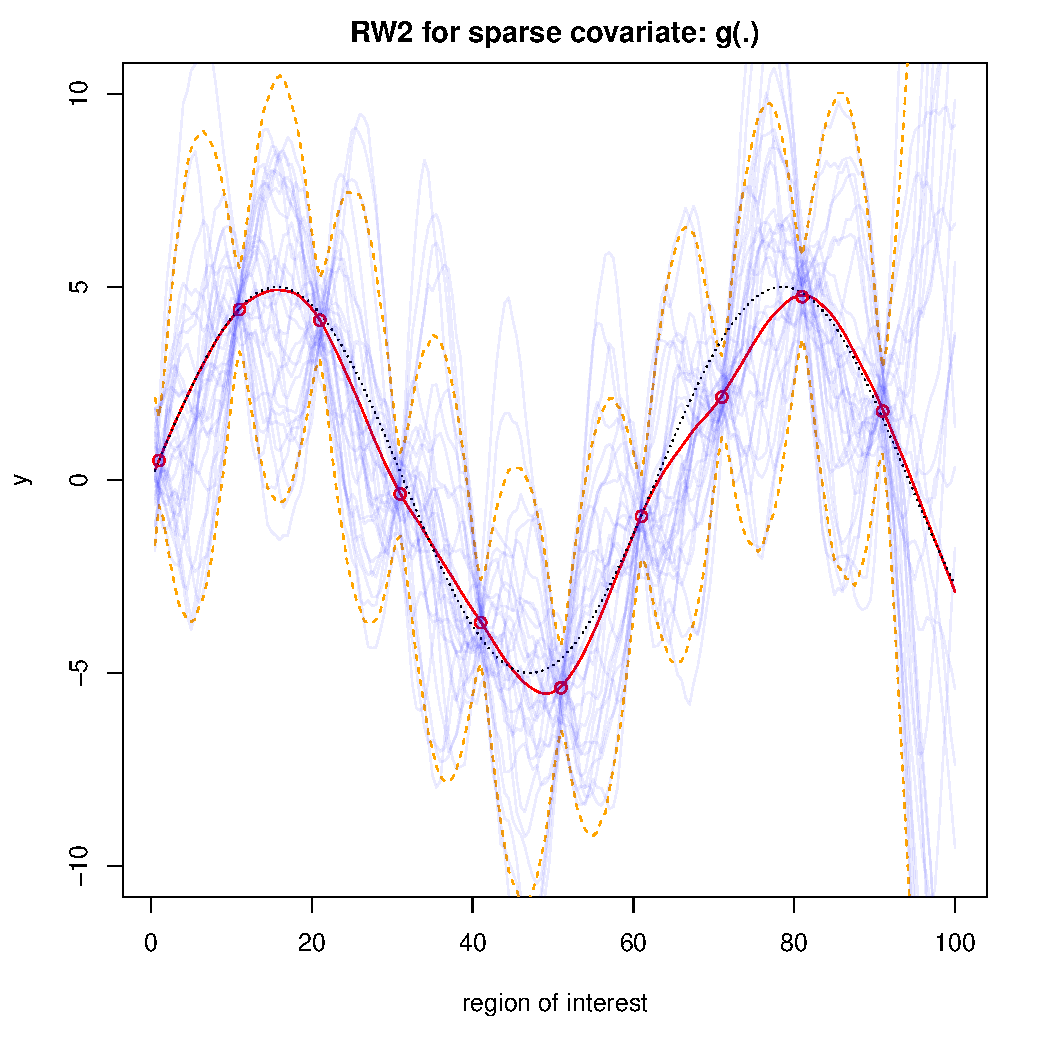
\includegraphics[width=0.47\textwidth]{sim1-g-RW2.pdf}
    }
    \subfigure[$g$ inferred using ARIMA]{
      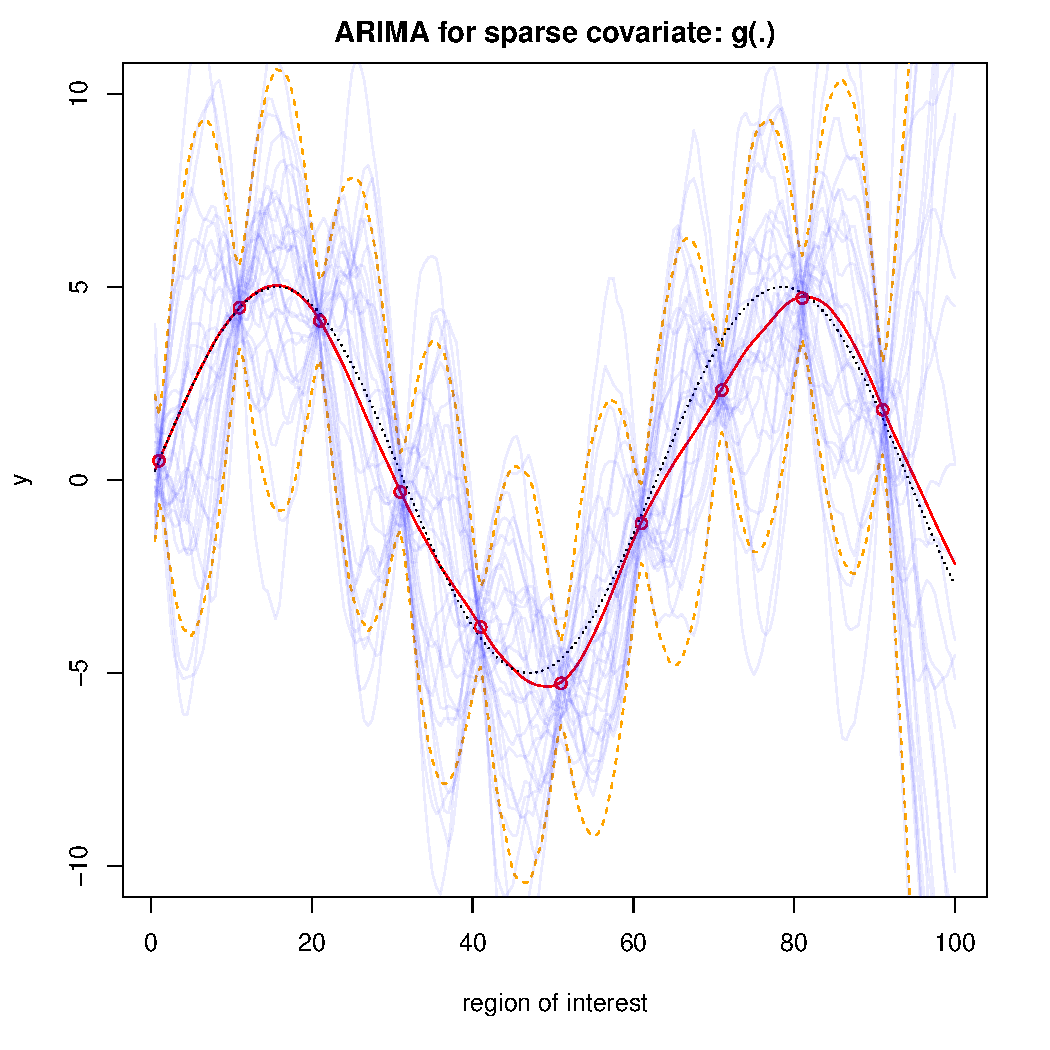
\includegraphics[width=0.47\textwidth]{sim1-g-ARIMA.pdf}
    }
    \subfigure[$g'$ inferred using RW2]{
      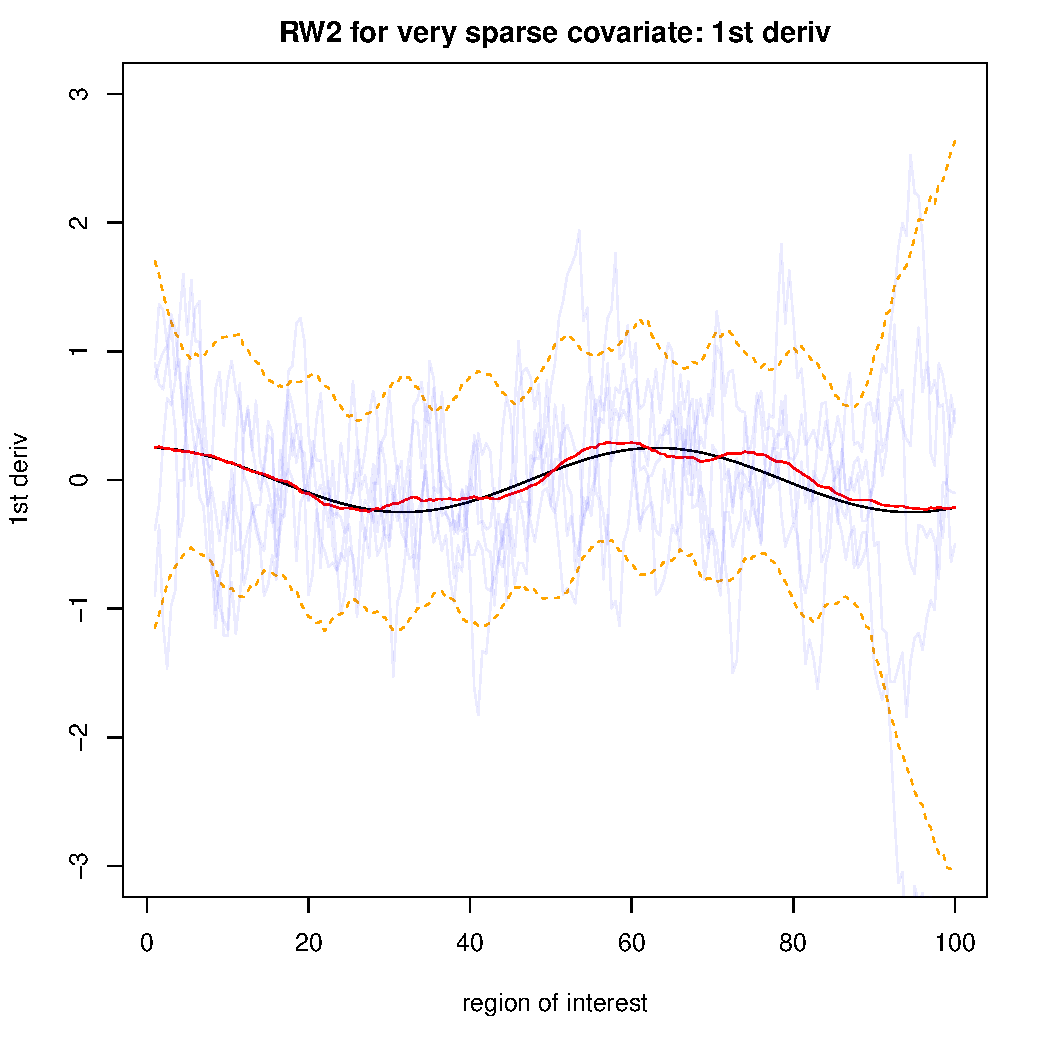
\includegraphics[width=0.47\textwidth]{sim1-g1st-RW2.pdf}
    }
     \subfigure[$g'$ inferred using ARIMA]{
      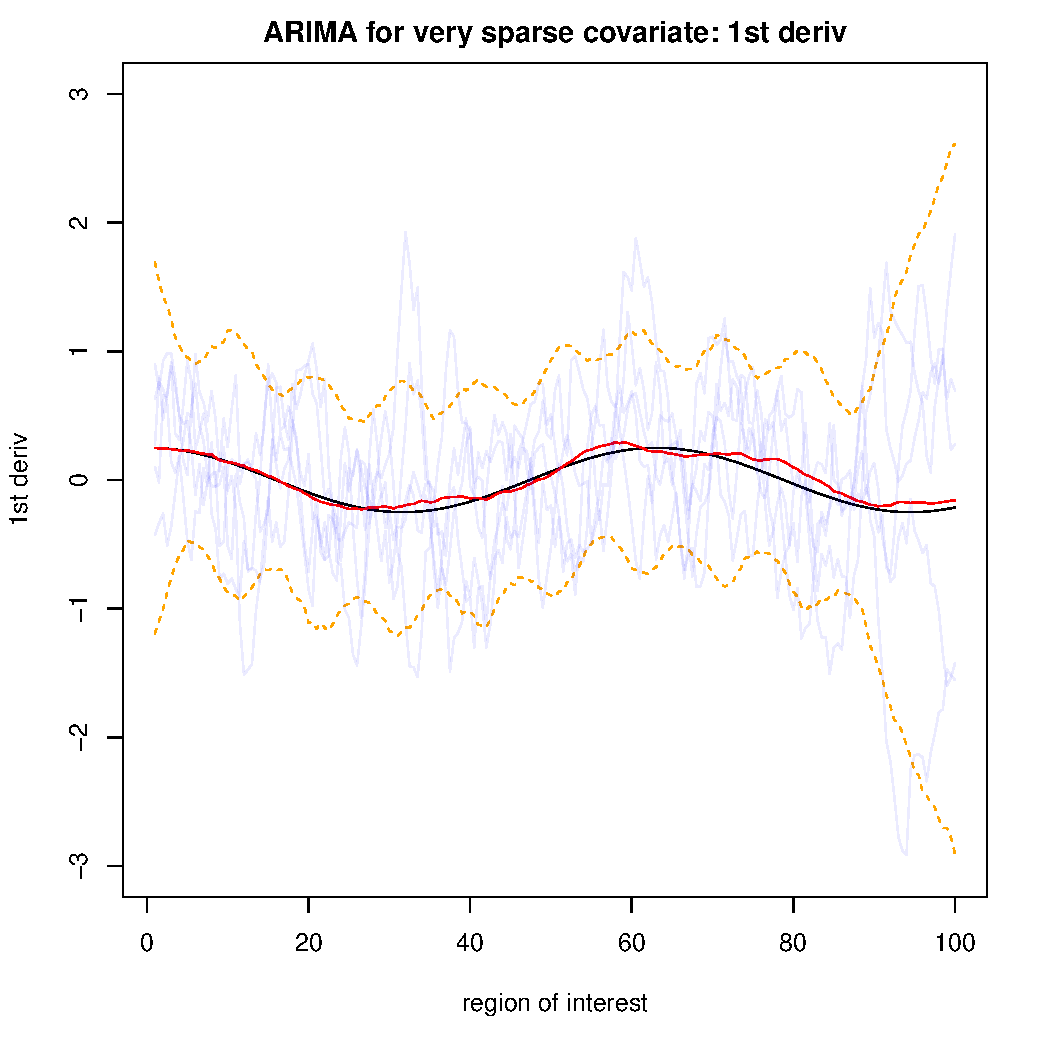
\includegraphics[width=0.47\textwidth]{sim1-g1st-ARIMA.pdf}
    }
        \subfigure[$g''$ inferred using RW2]{
      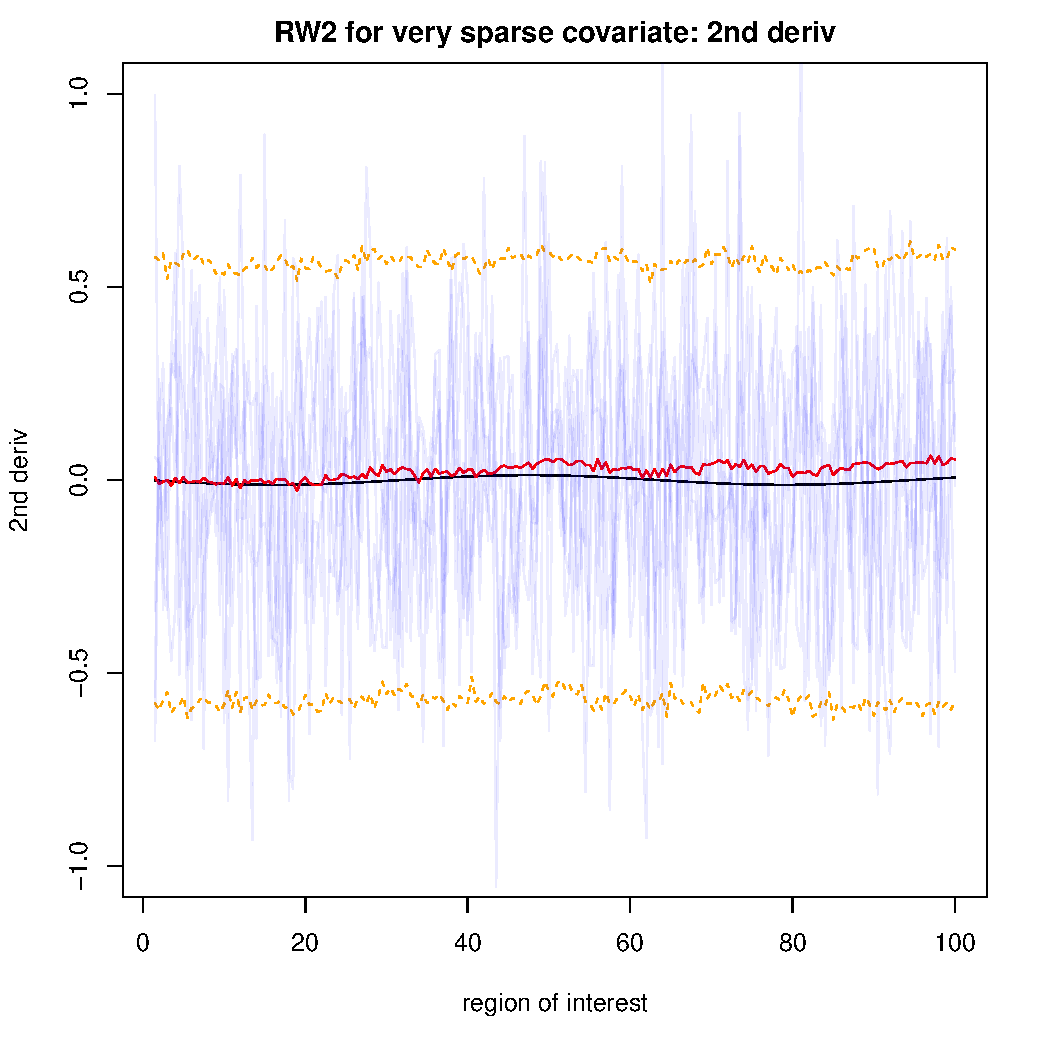
\includegraphics[width=0.47\textwidth]{sim1-g2nd-RW2.pdf}
    }
     \subfigure[$g''$ inferred using ARIMA]{
      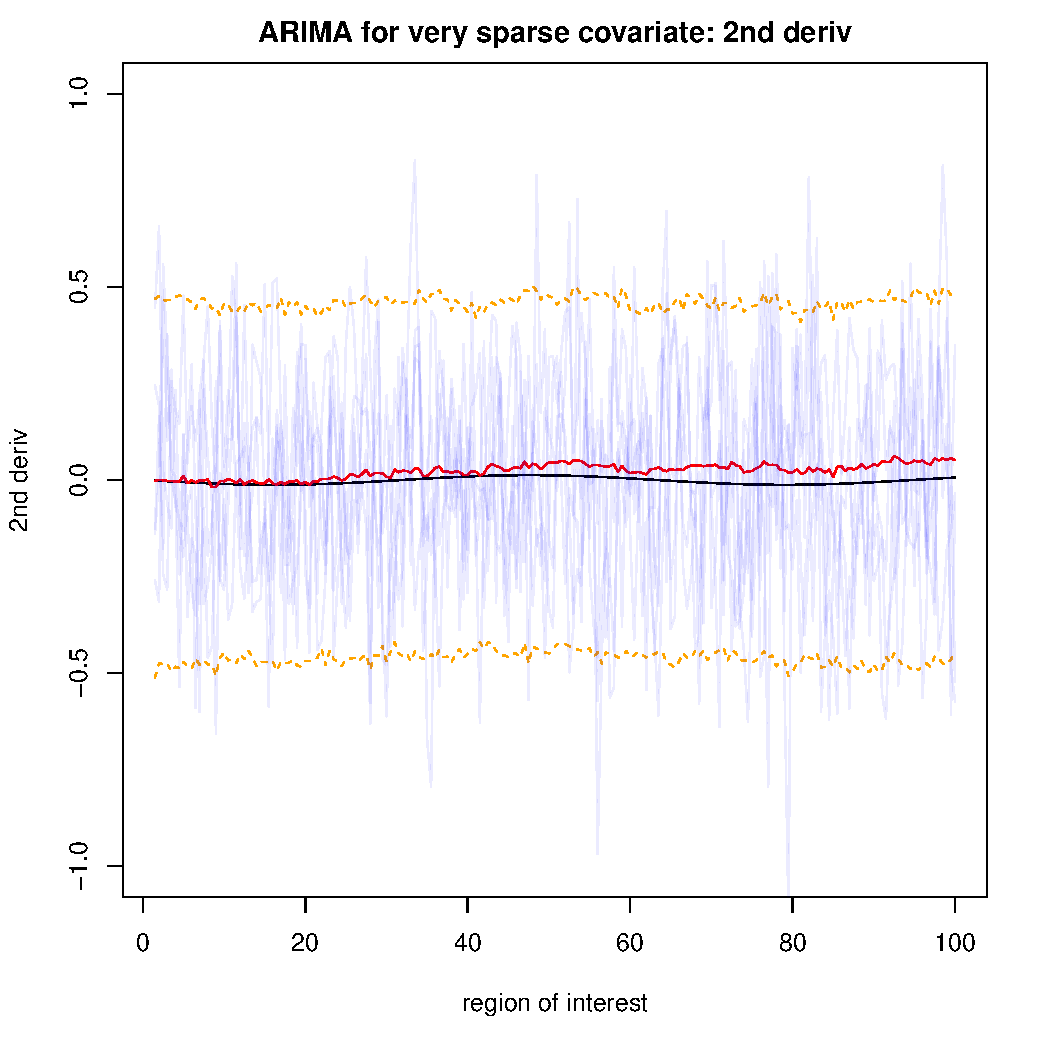
\includegraphics[width=0.47\textwidth]{sim1-g2nd-ARIMA.pdf}
    }
    \caption{Inference for $g,g',g''$ using different methods for simulation 1; The light blue lines are samples from the posterior distribution; The red lines are posterior mean; The orange lines are the posterior credible interval with 90 percent coverage rate; The black line is the true value.}
    \label{fig:sim1-1replic}
\end{figure}


\begin{figure}[p]
    \centering
    \subfigure[rIAE for $g$]{
      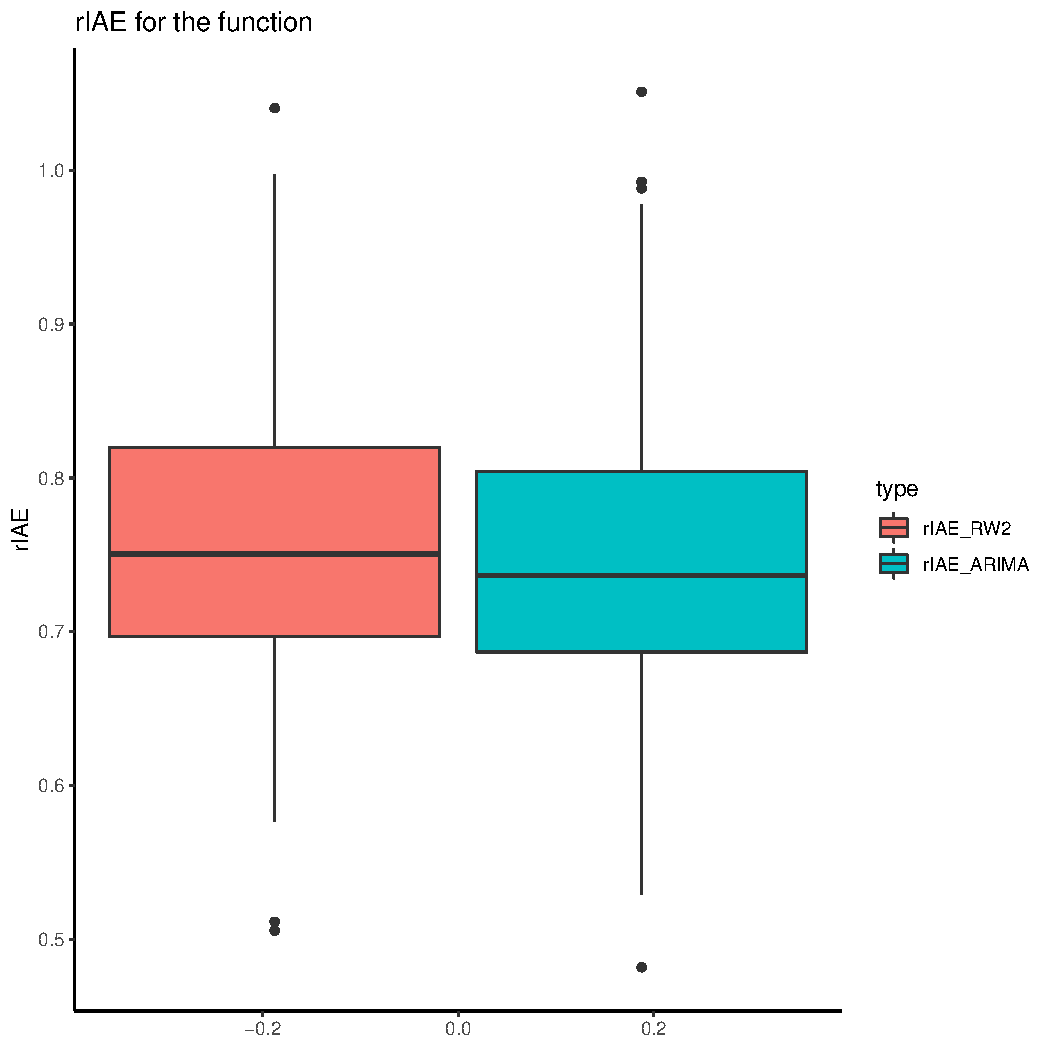
\includegraphics[width=0.29\textwidth]{sim1-g-rIAE.pdf}
    }
    \subfigure[MCI for $g$]{
      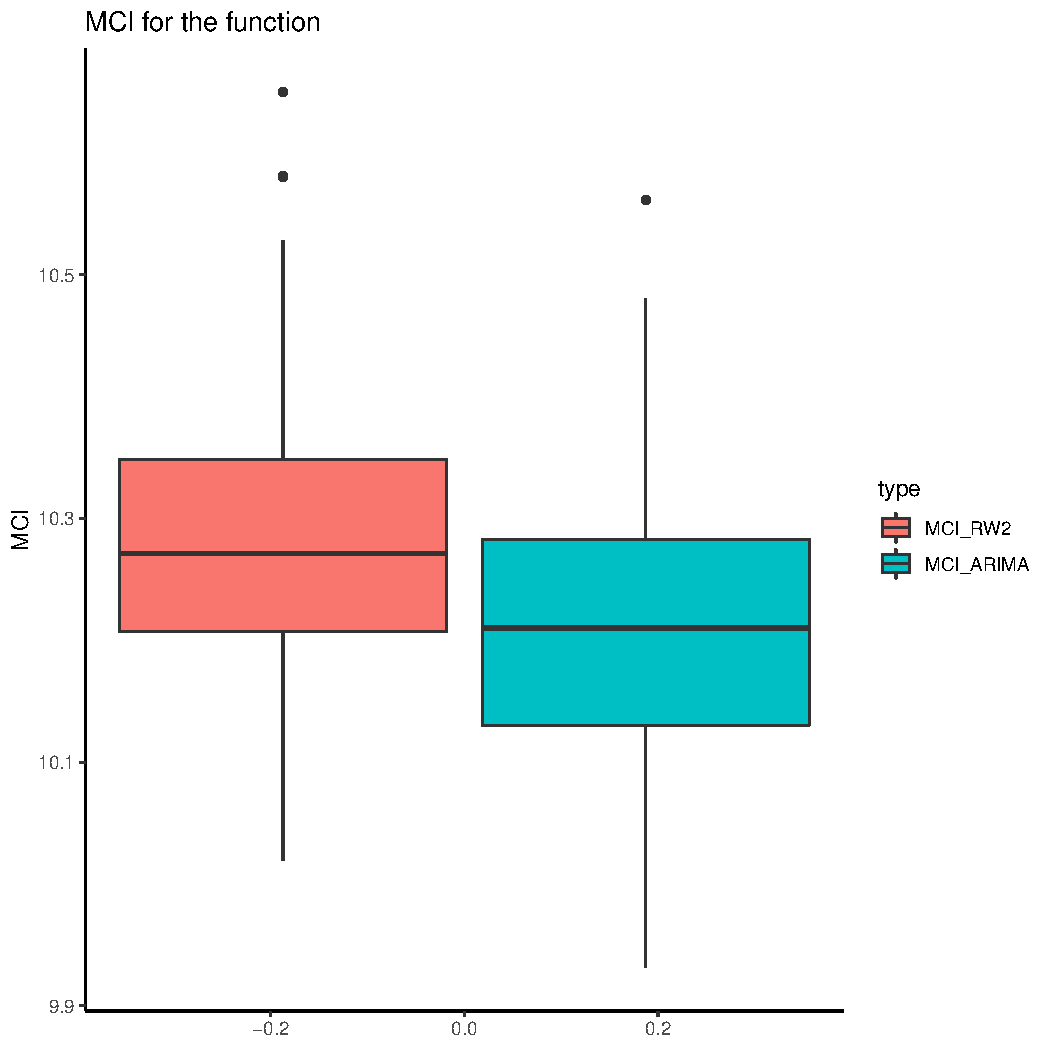
\includegraphics[width=0.29\textwidth]{sim1-g-MCI.pdf}
    }
    \subfigure[CR for $g$]{
      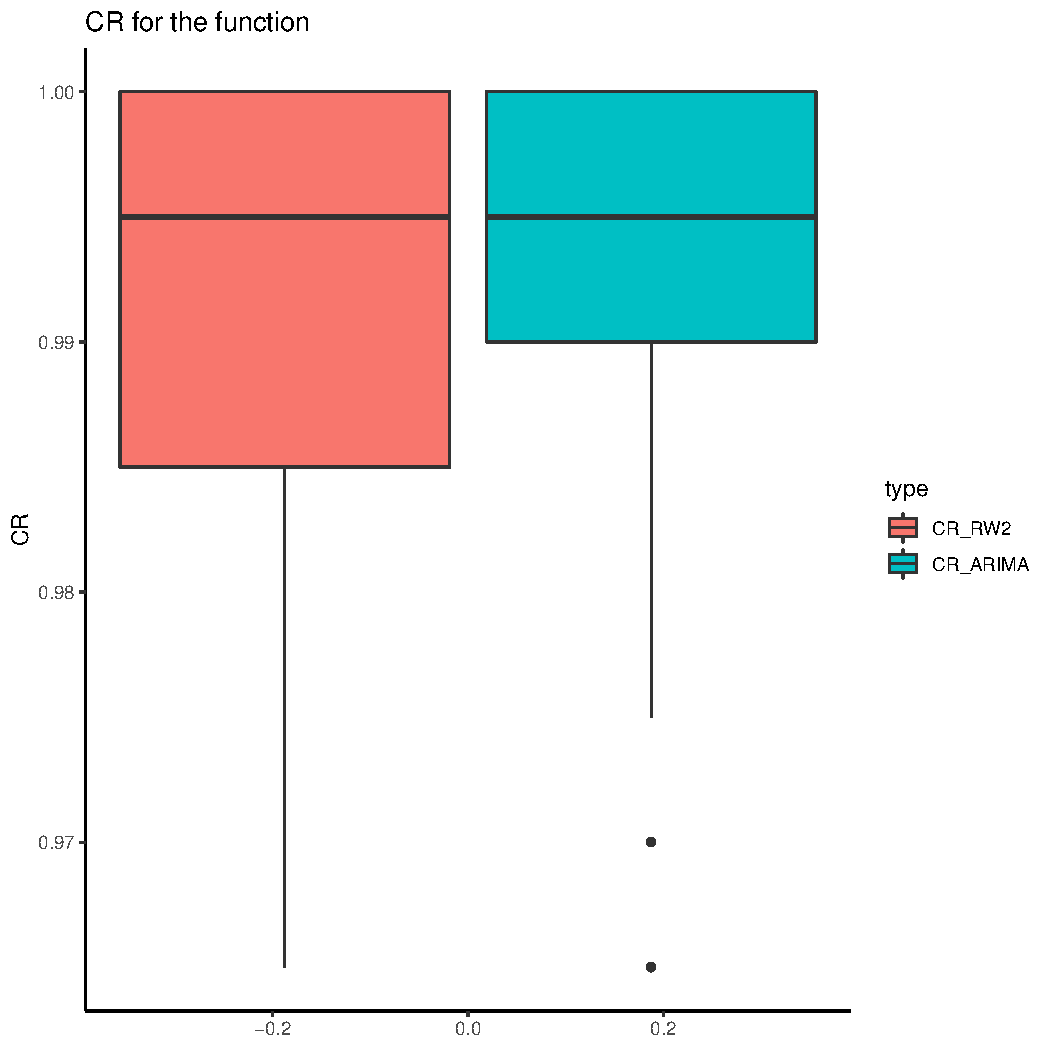
\includegraphics[width=0.29\textwidth]{sim1-g-CR.pdf}
    }
     \subfigure[rIAE for $g'$]{
      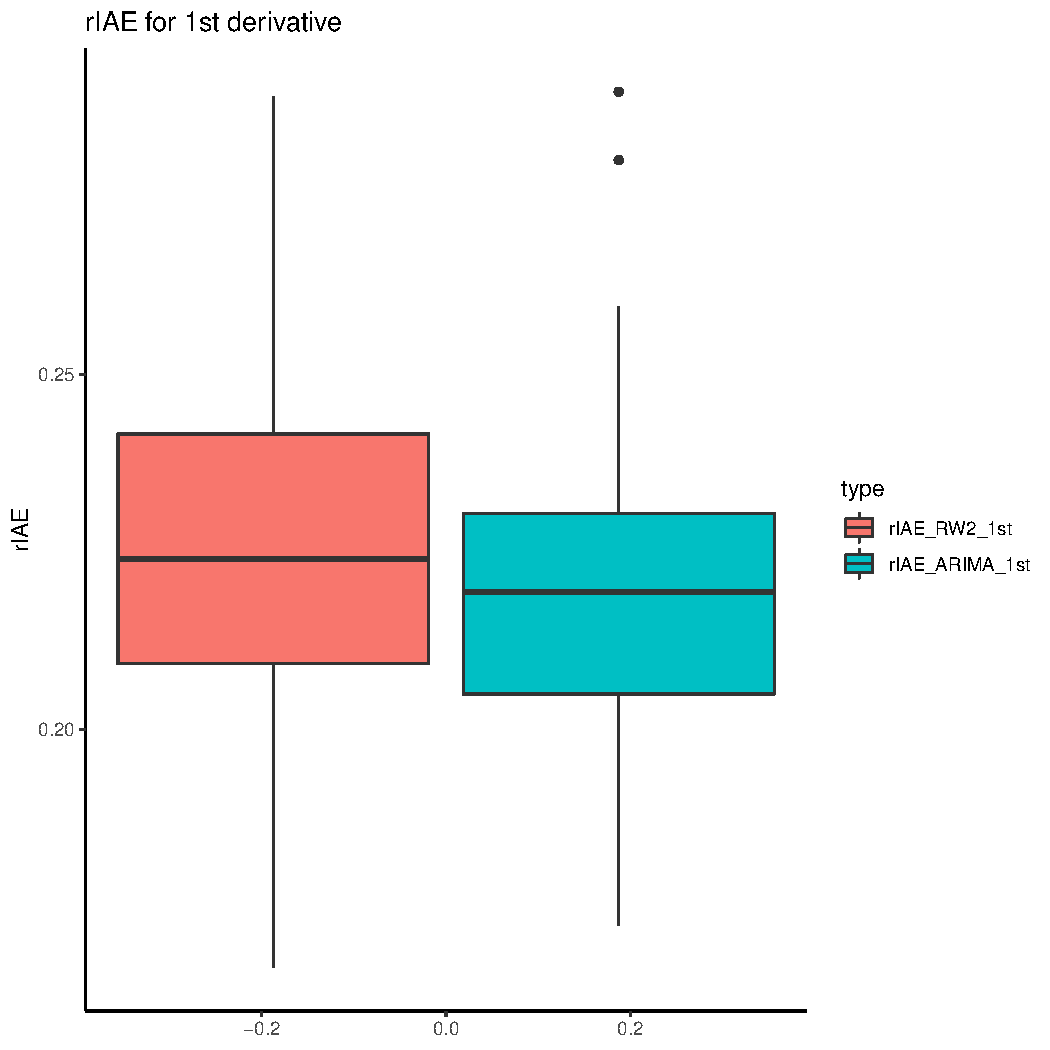
\includegraphics[width=0.29\textwidth]{sim1-g1st-rIAE.pdf}
    }
        \subfigure[MCI for $g'$]{
      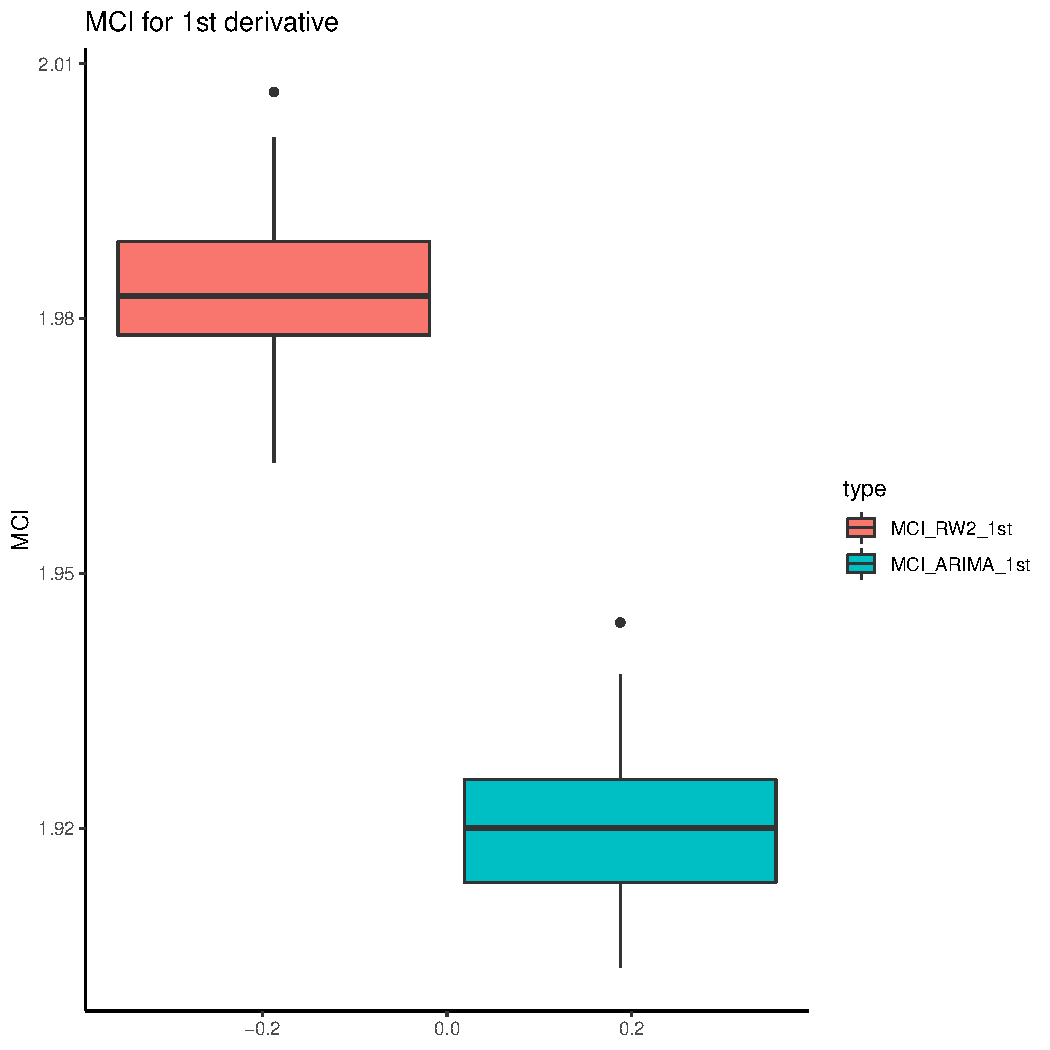
\includegraphics[width=0.29\textwidth]{sim1-g1st-MCI.pdf}
    }
     \subfigure[CR for $g'$]{
      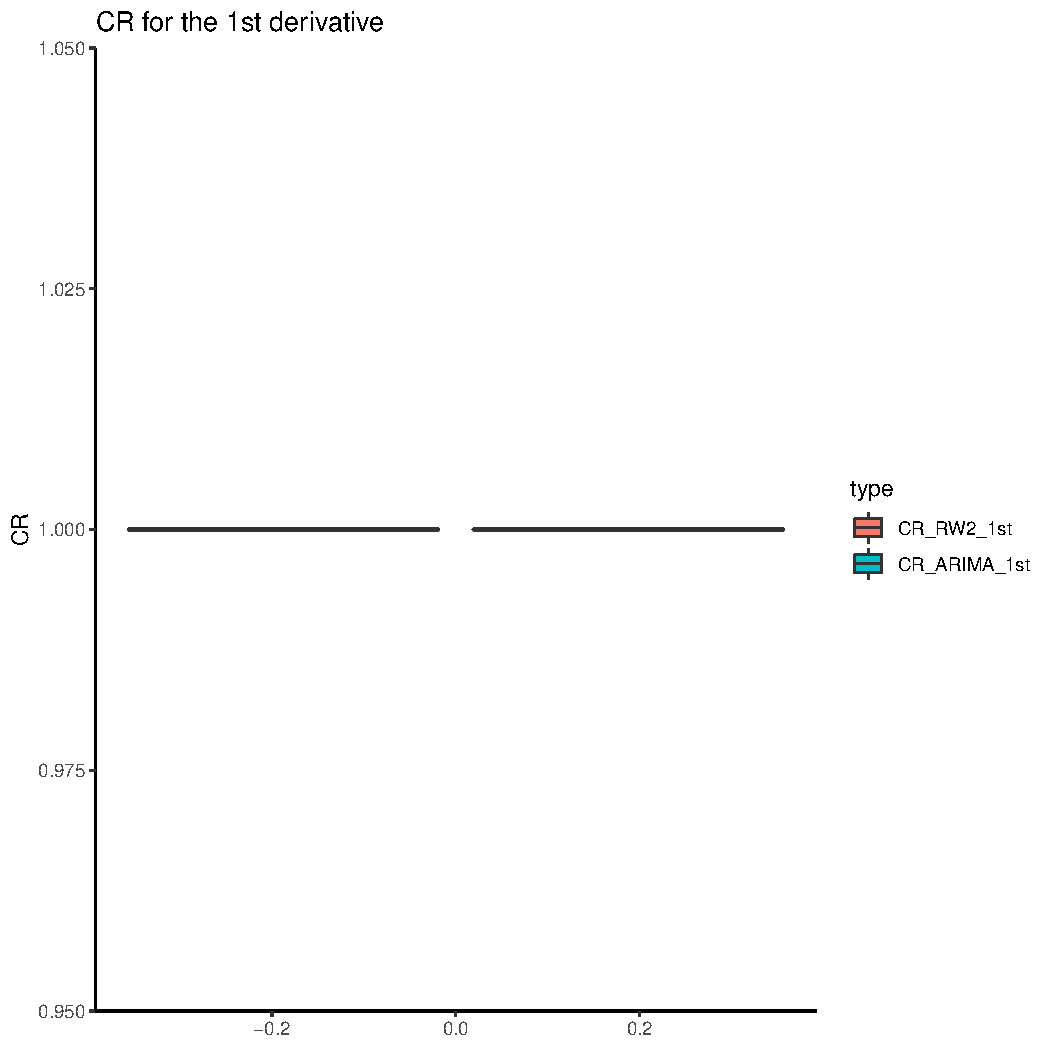
\includegraphics[width=0.29\textwidth]{sim1-g1st-CR.pdf}
    }
         \subfigure[rIAE for $g''$]{
      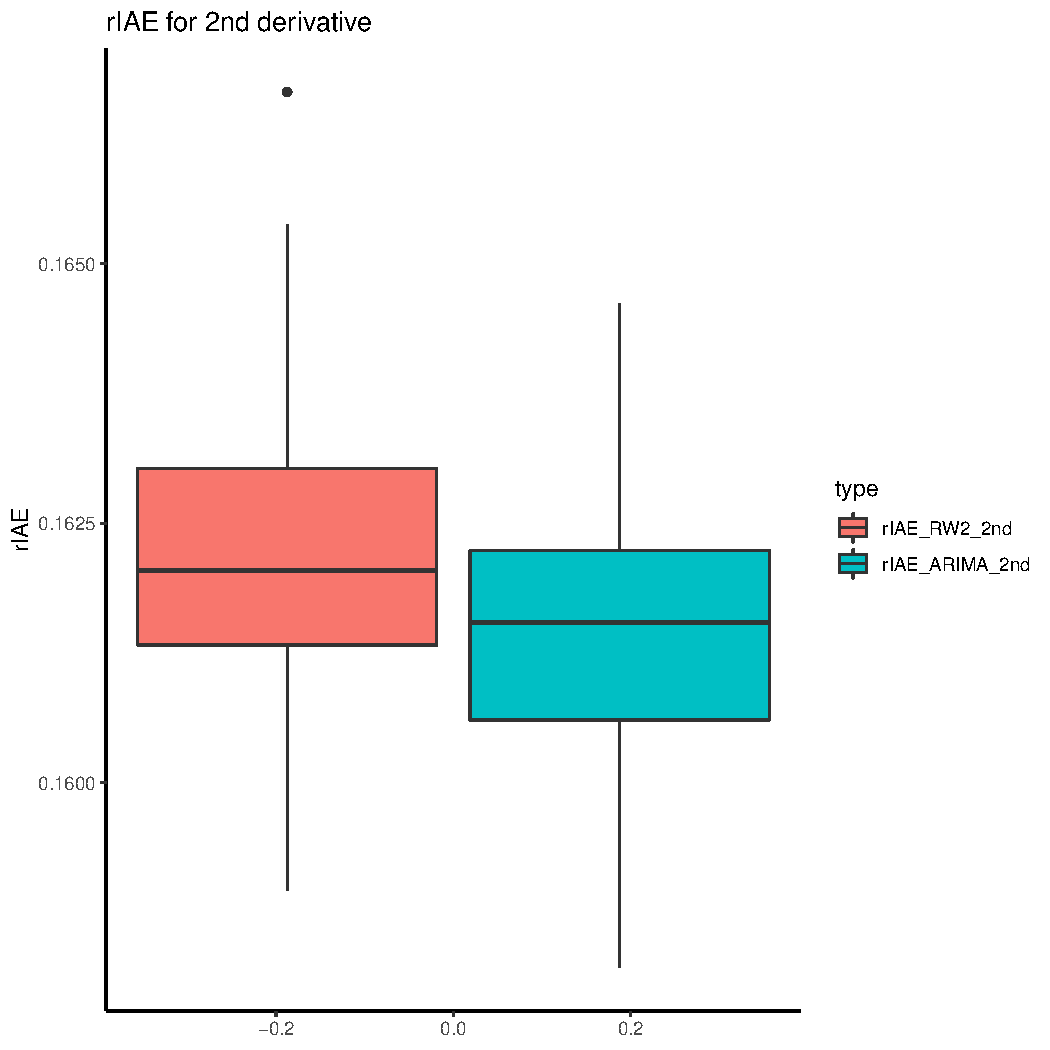
\includegraphics[width=0.29\textwidth]{sim1-g2nd-rIAE.pdf}
    }
        \subfigure[MCI for $g''$]{
      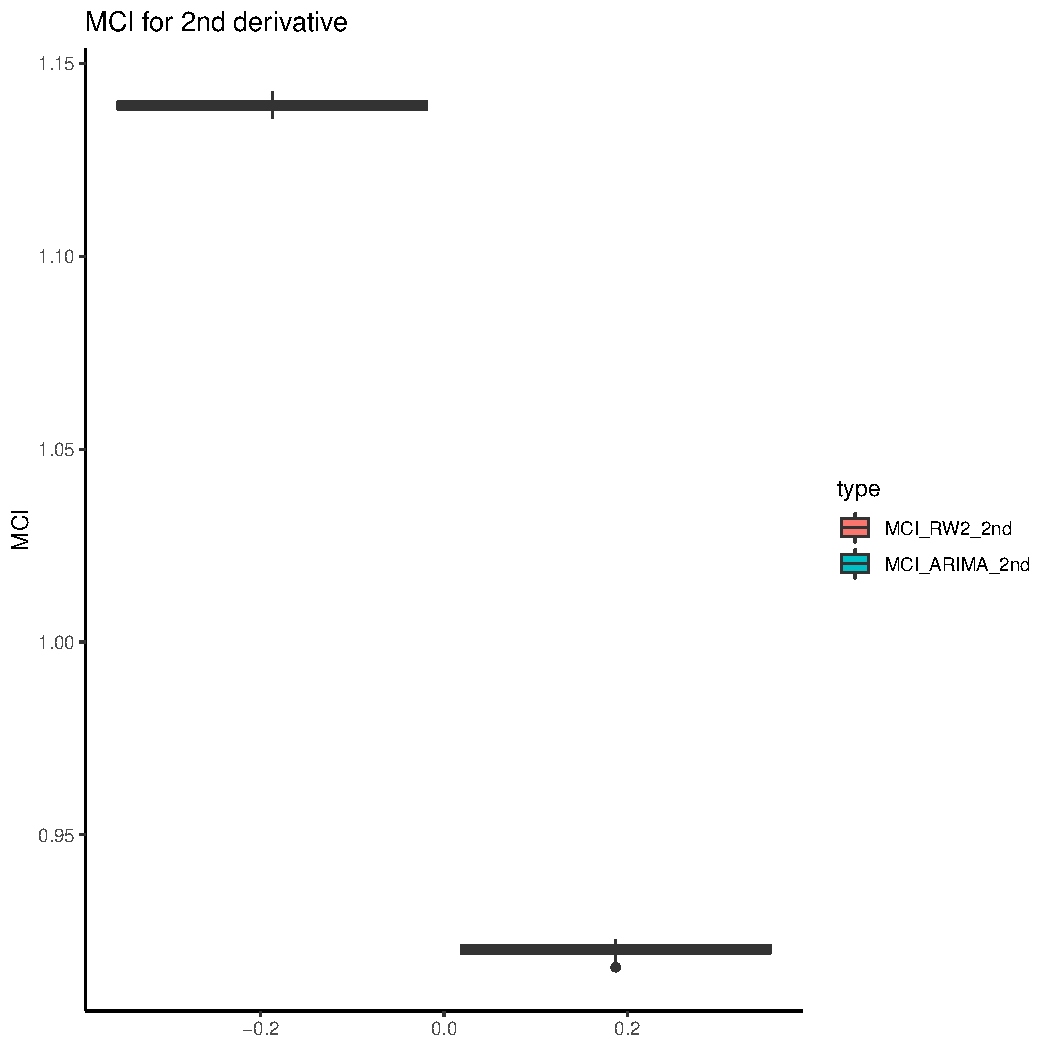
\includegraphics[width=0.29\textwidth]{sim1-g2nd-MCI.pdf}
    }
     \subfigure[CR for $g''$]{
      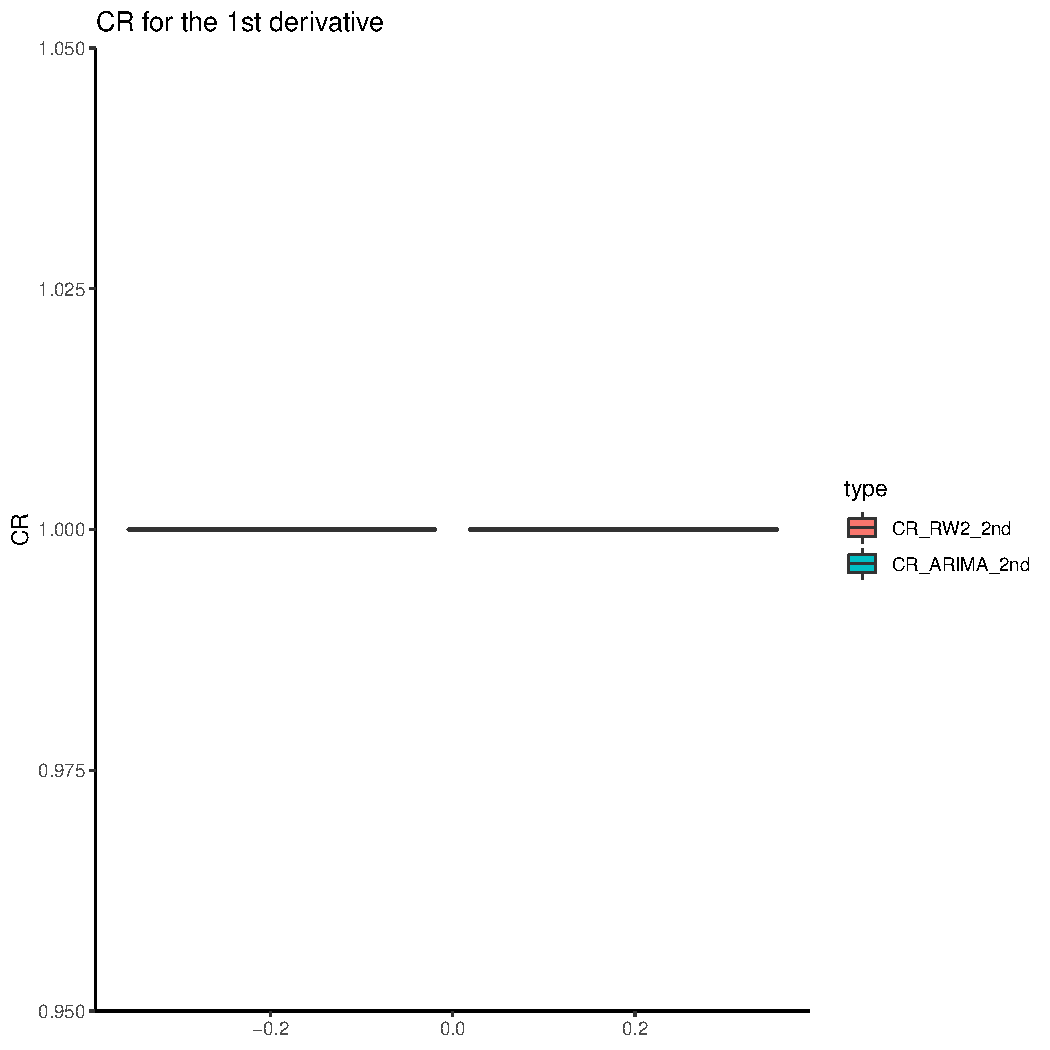
\includegraphics[width=0.29\textwidth]{sim1-g2nd-CR.pdf}
    }
    \caption{Inference for $g,g',g''$ using different methods for simulation 1, being replicated for 100 independent data sets.}
    \label{fig:sim1-100replic}
\end{figure}



\begin{figure}[p]
    \centering
    \subfigure[$g$ inferred using RW2]{
      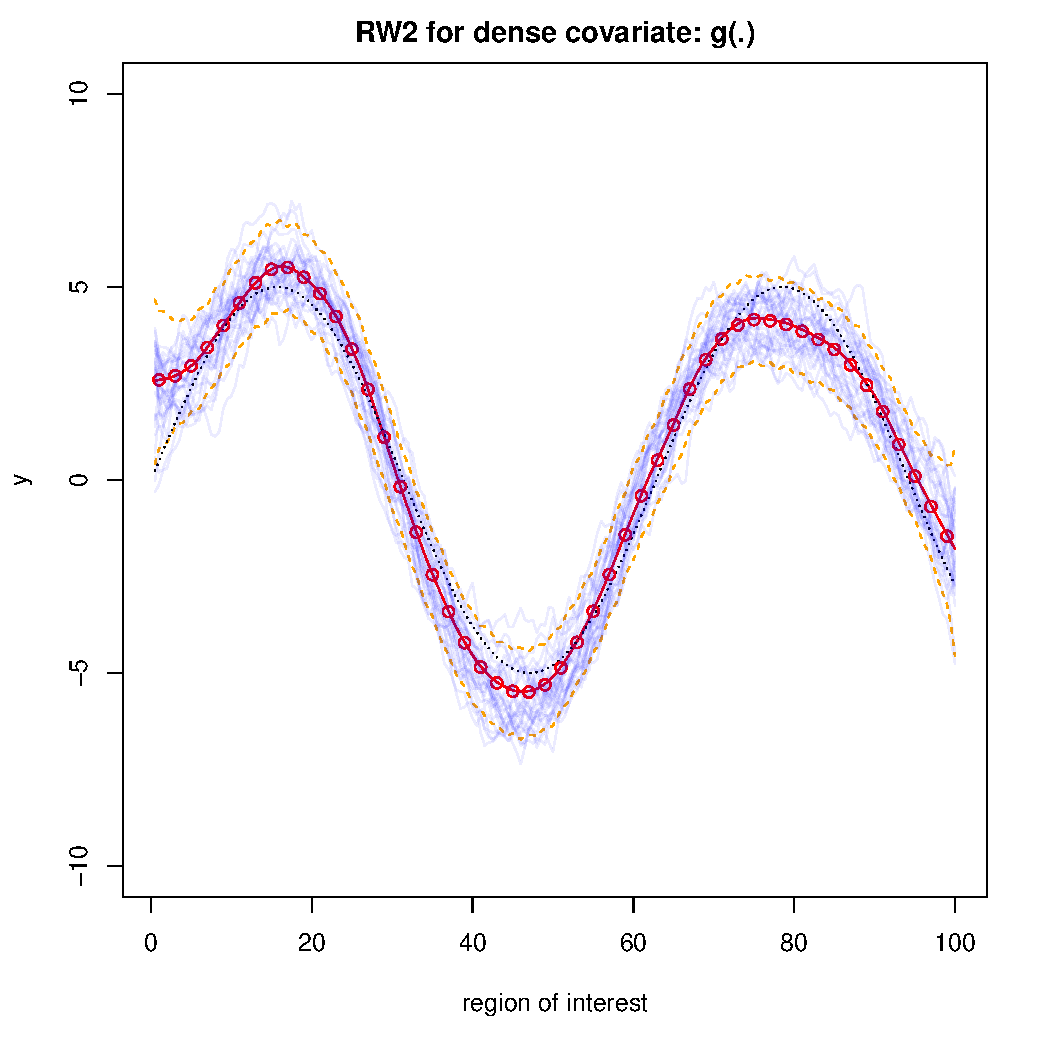
\includegraphics[width=0.47\textwidth]{sim2-g-RW2.pdf}
    }
    \subfigure[$g$ inferred using ARIMA]{
      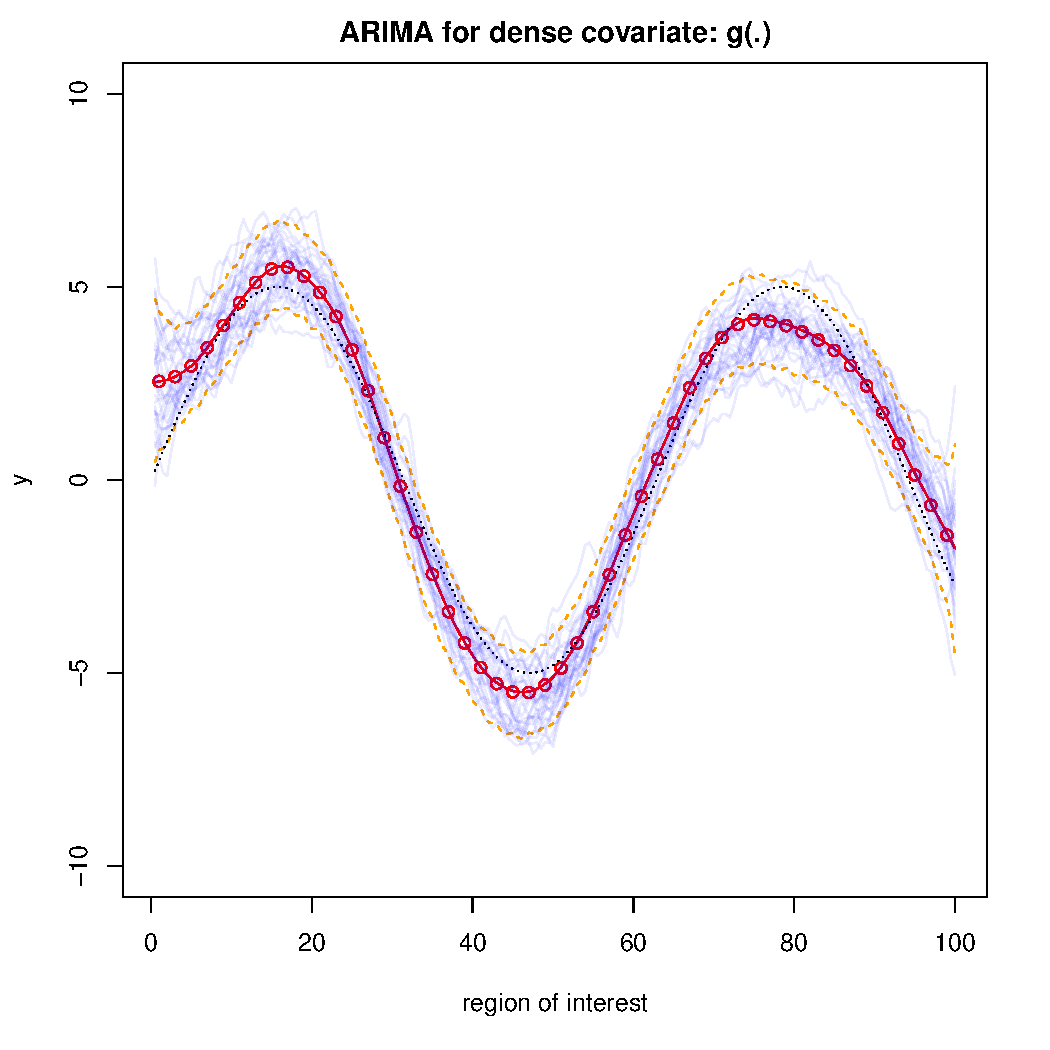
\includegraphics[width=0.47\textwidth]{sim2-g-ARIMA.pdf}
    }
    \subfigure[$g'$ inferred using RW2]{
      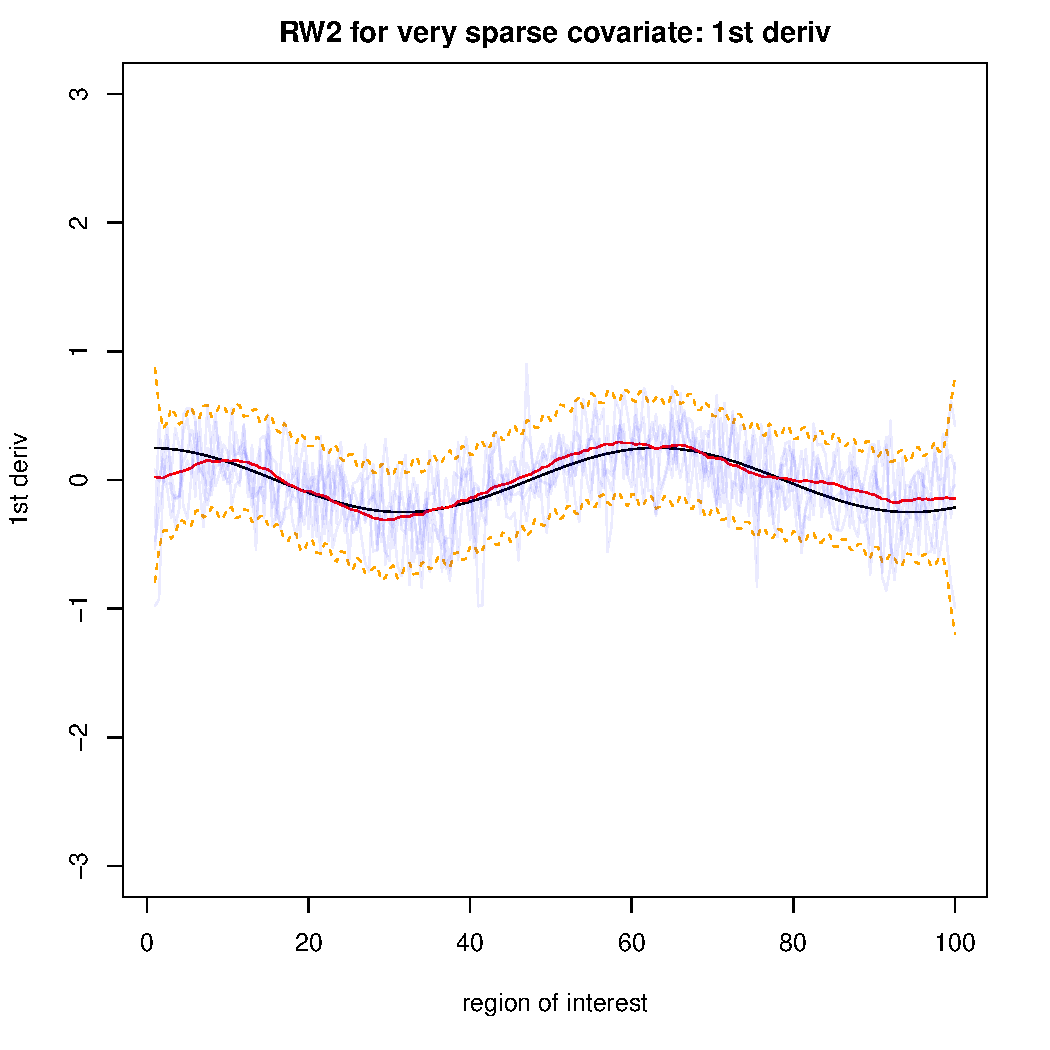
\includegraphics[width=0.47\textwidth]{sim2-g1st-RW2.pdf}
    }
     \subfigure[$g'$ inferred using ARIMA]{
      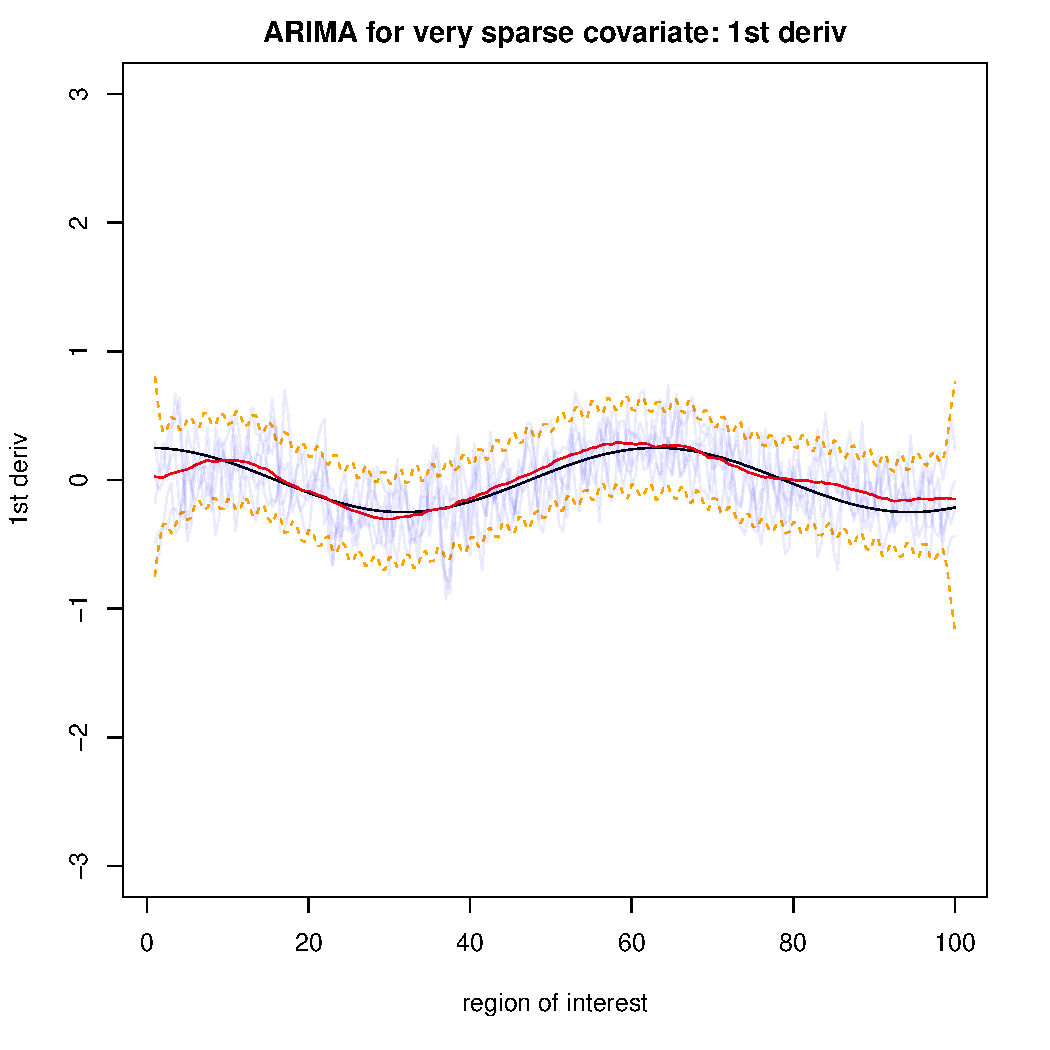
\includegraphics[width=0.47\textwidth]{sim2-g1st-ARIMA.pdf}
    }
        \subfigure[$g''$ inferred using RW2]{
      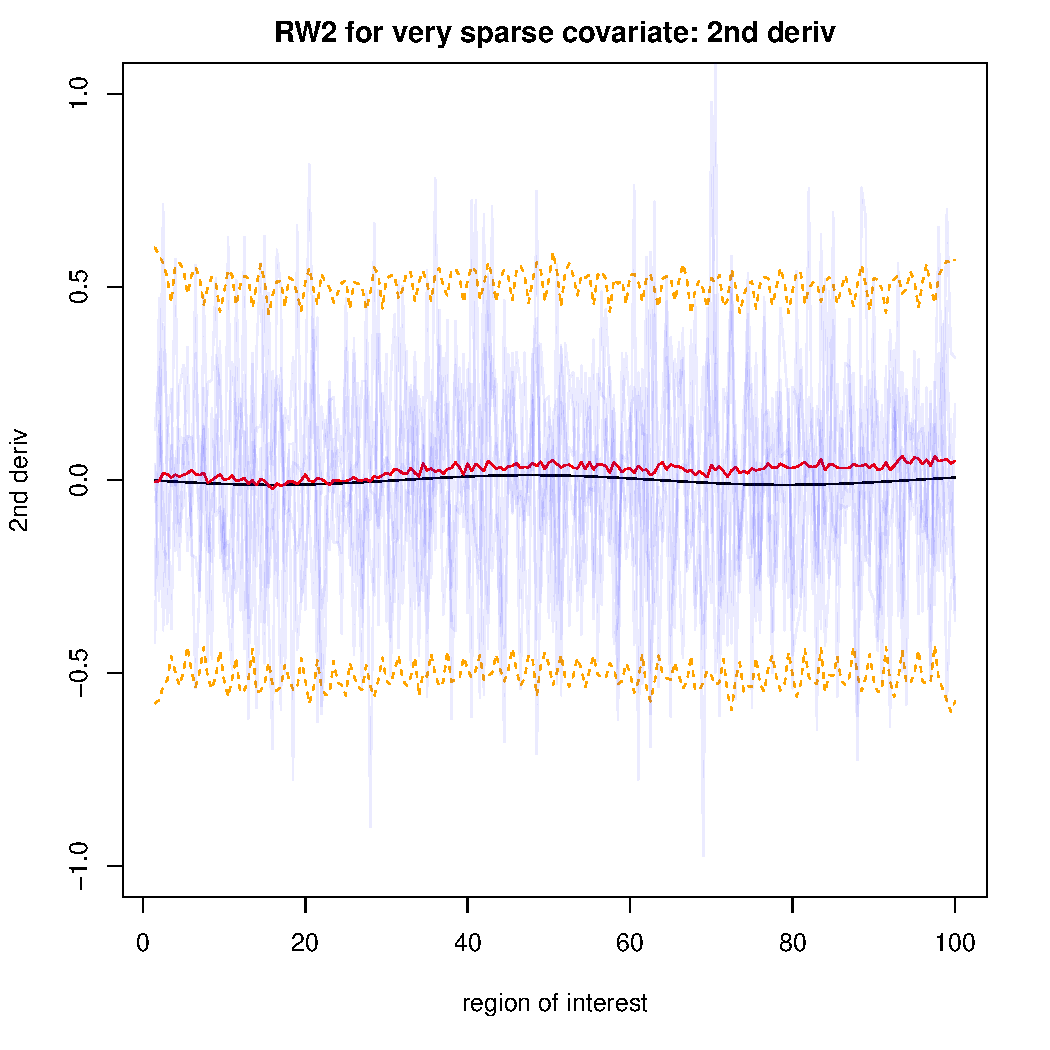
\includegraphics[width=0.47\textwidth]{sim2-g2nd-RW2.pdf}
    }
     \subfigure[$g''$ inferred using ARIMA]{
      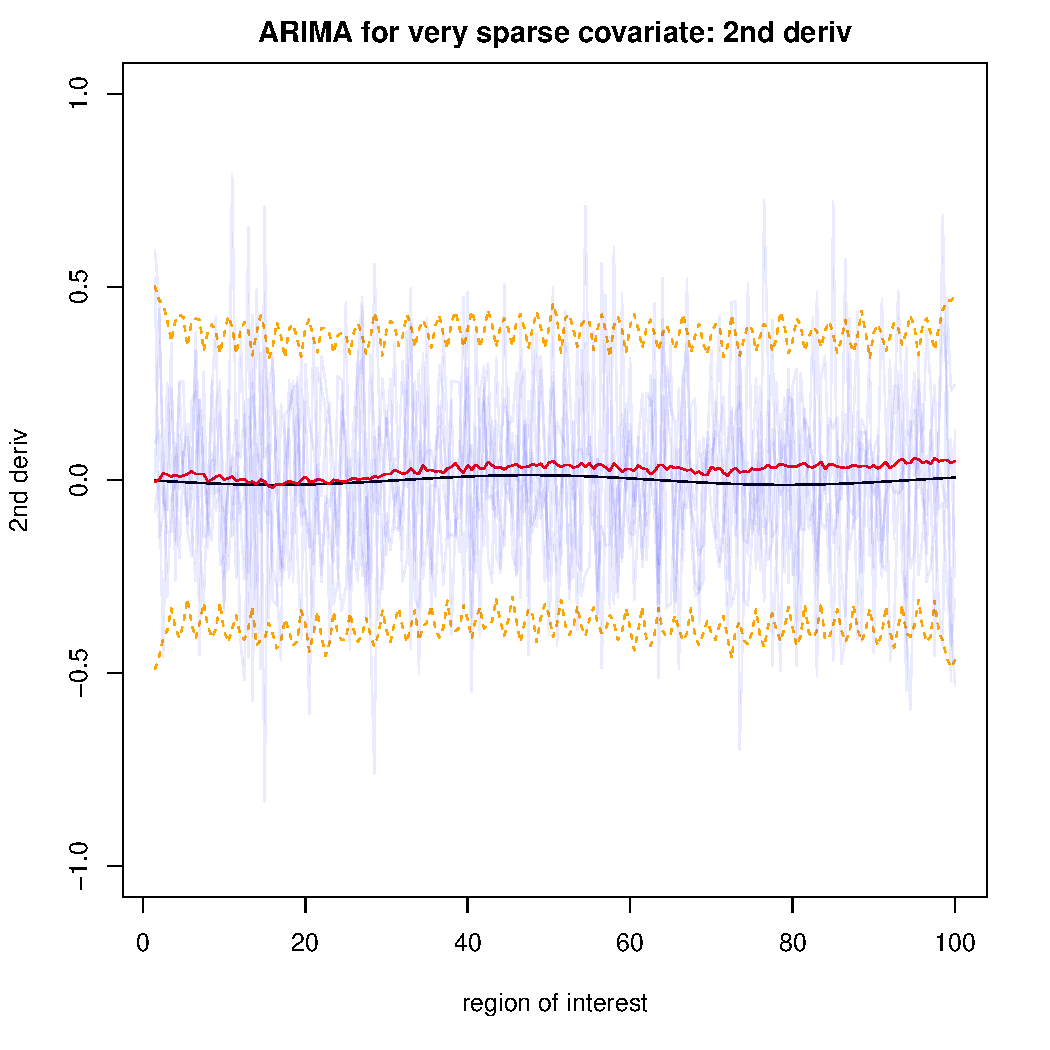
\includegraphics[width=0.47\textwidth]{sim2-g2nd-ARIMA.pdf}
    }
    \caption{Inference for $g,g',g''$ using different methods for simulation 2; The light blue lines are samples from the posterior distribution; The red lines are posterior mean; The orange lines are the posterior credible interval with 90 percent coverage rate; The black line is the true value.}
    \label{fig:sim2-1replic}
\end{figure}



\begin{figure}[p]
    \centering
    \subfigure[rIAE for $g$]{
      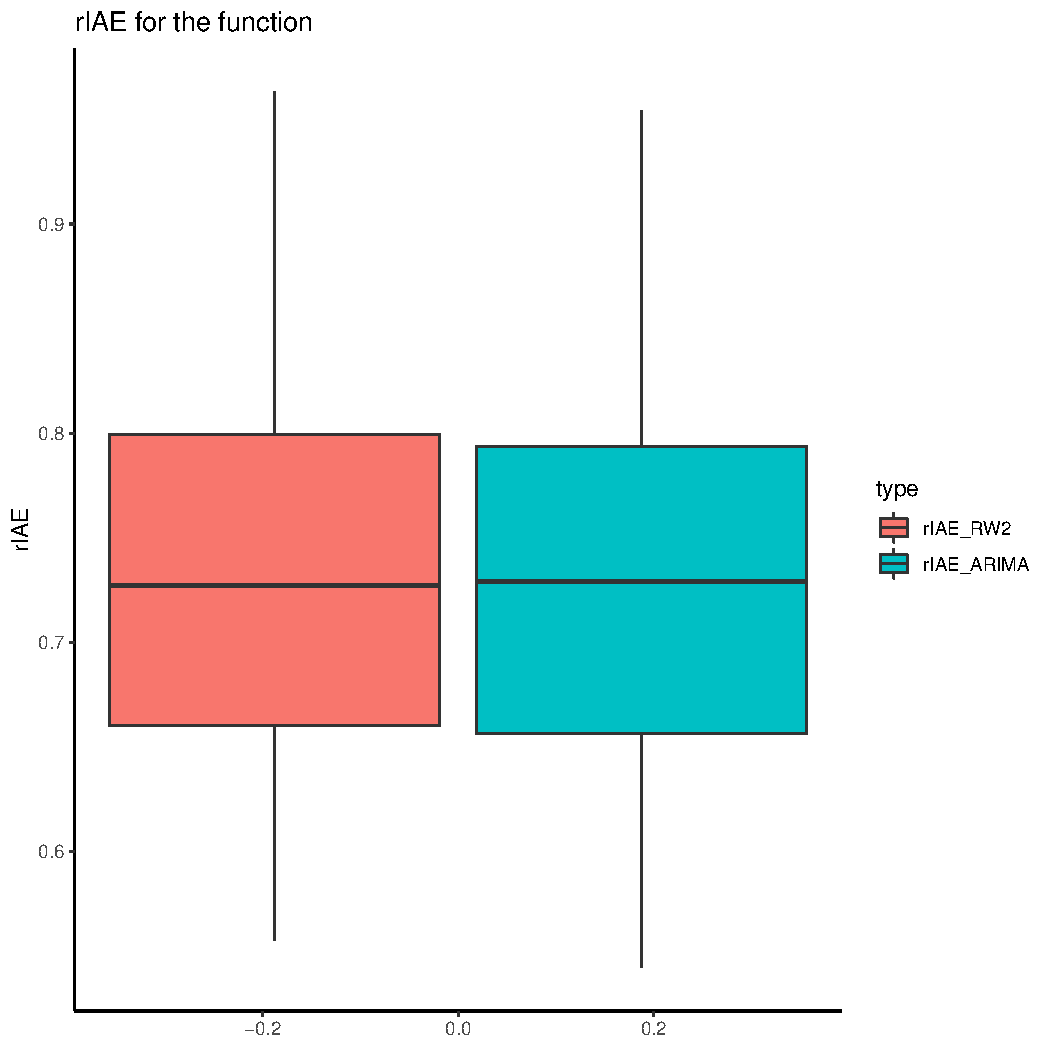
\includegraphics[width=0.29\textwidth]{sim2-g-rIAE.pdf}
    }
    \subfigure[MCI for $g$]{
      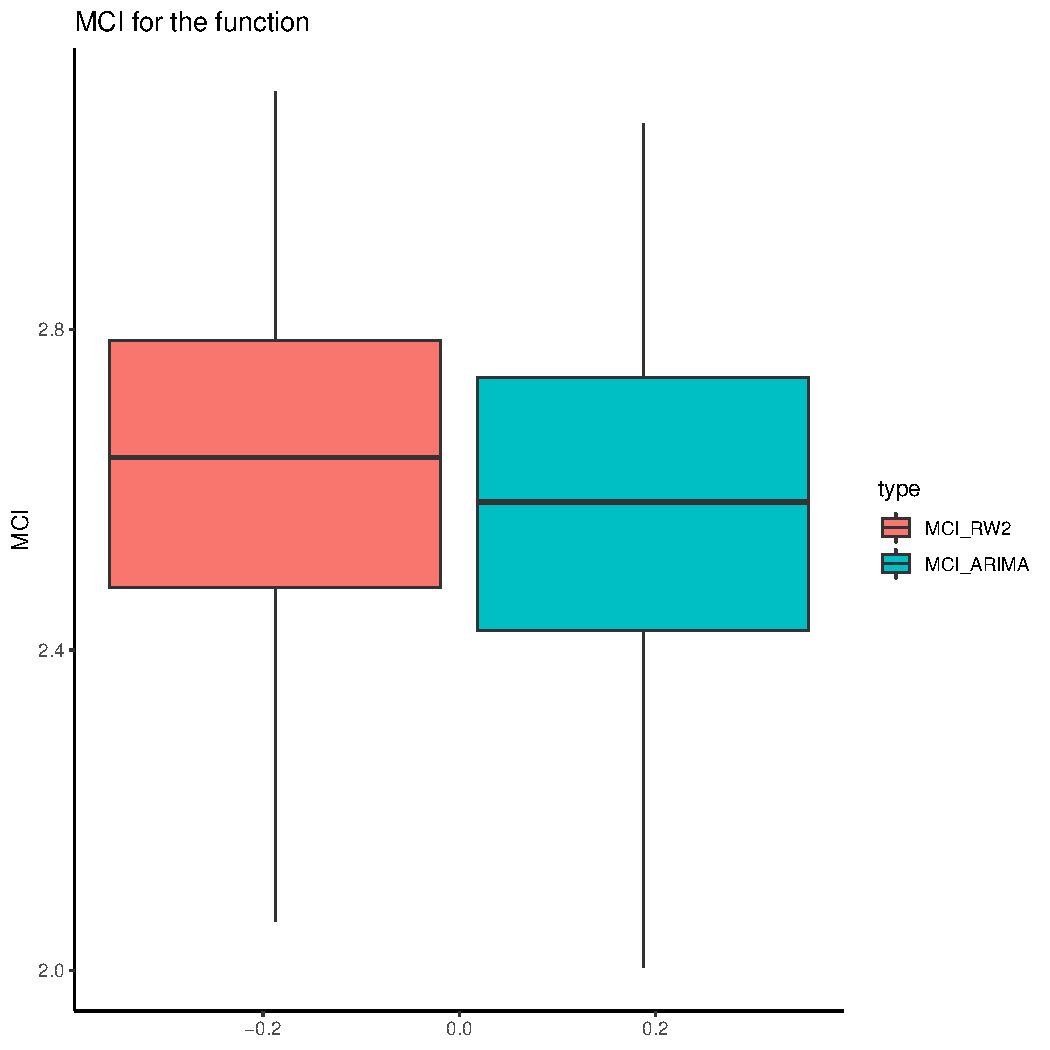
\includegraphics[width=0.29\textwidth]{sim2-g-MCI.pdf}
    }
    \subfigure[CR for $g$]{
      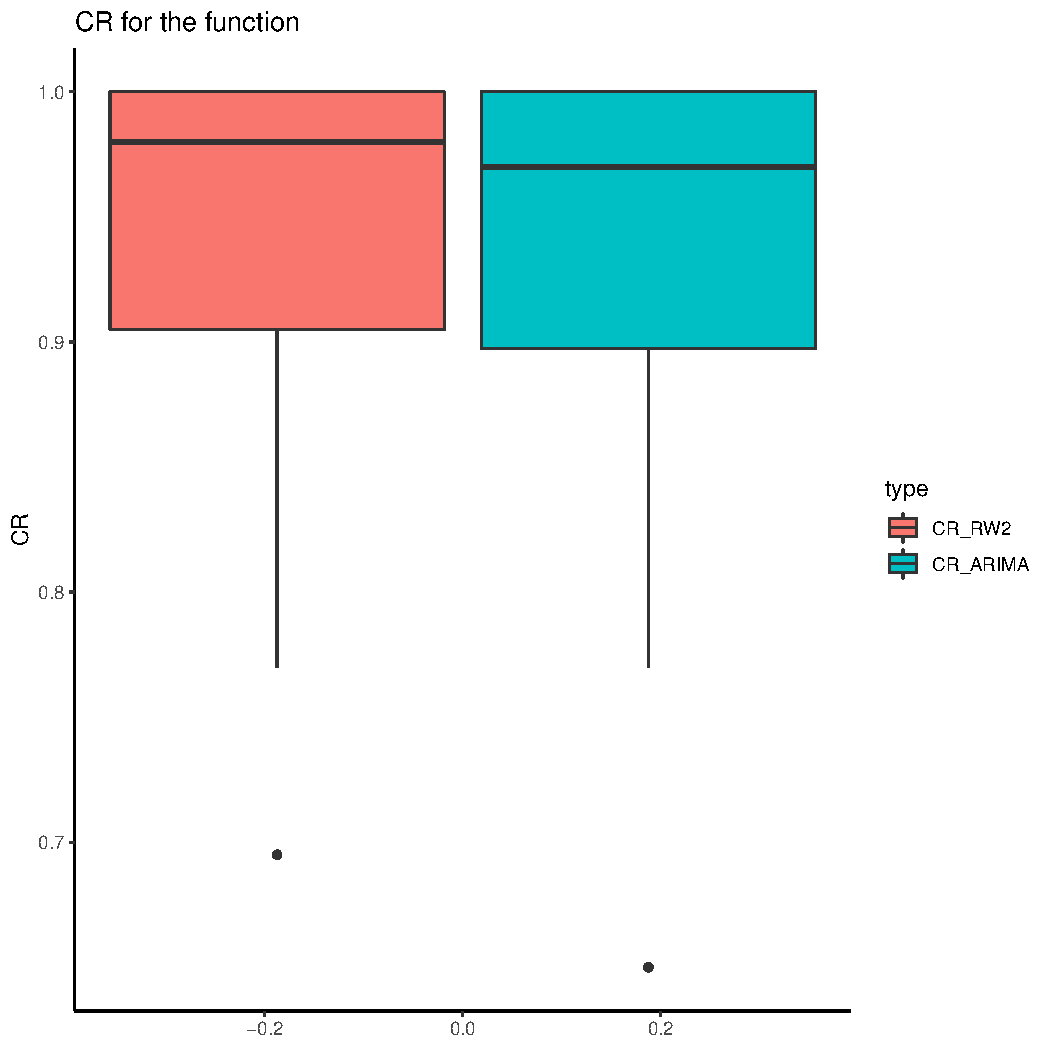
\includegraphics[width=0.29\textwidth]{sim2-g-CR.pdf}
    }
     \subfigure[rIAE for $g'$]{
      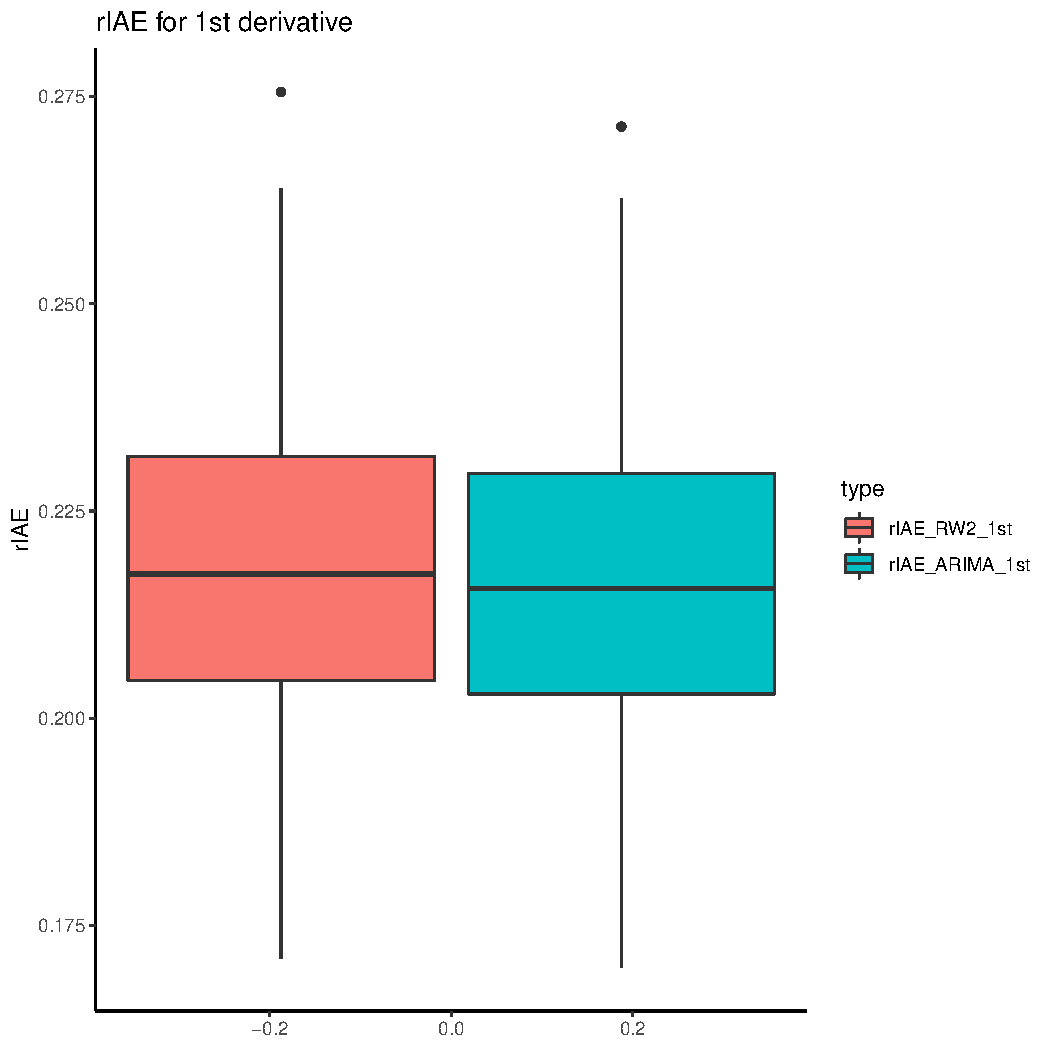
\includegraphics[width=0.29\textwidth]{sim2-g1st-rIAE.pdf}
    }
        \subfigure[MCI for $g'$]{
      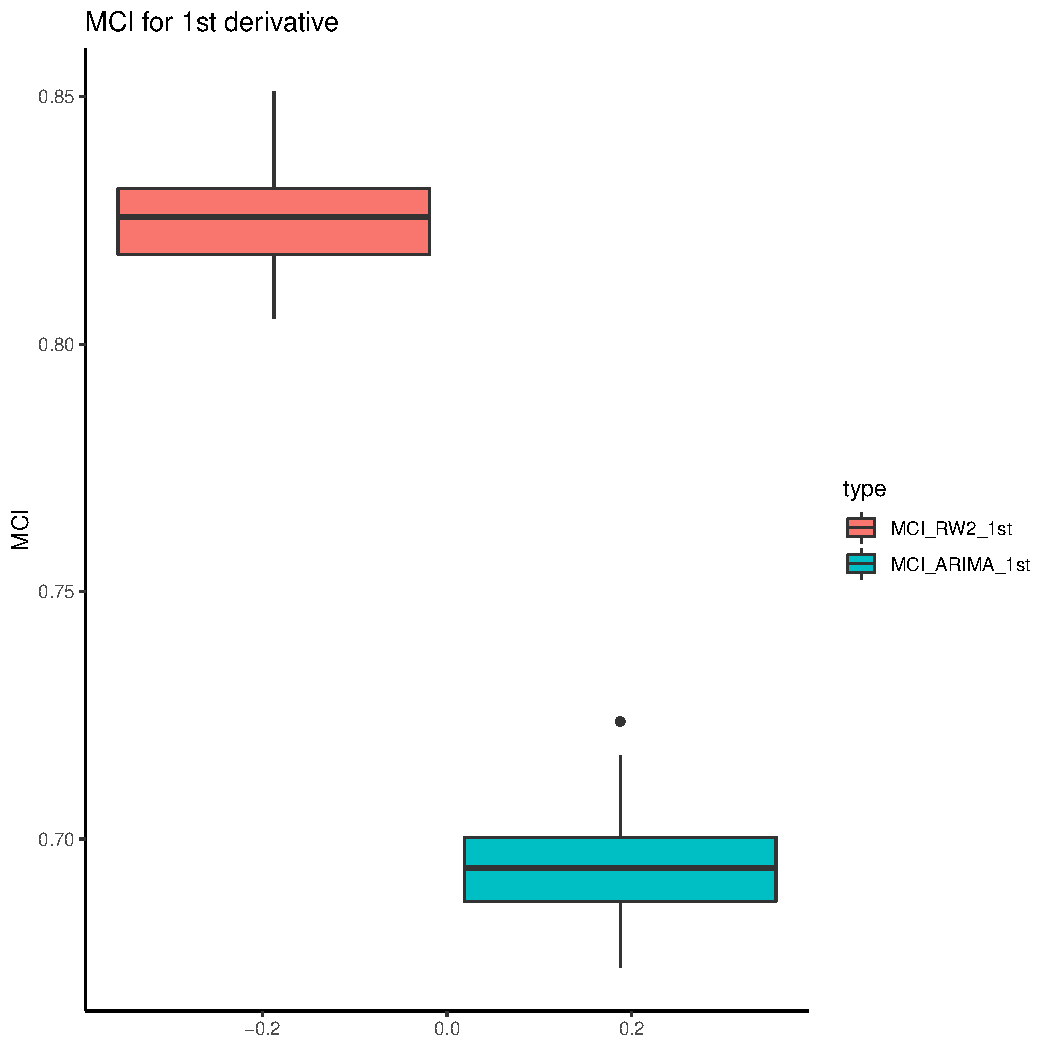
\includegraphics[width=0.29\textwidth]{sim2-g1st-MCI.pdf}
    }
     \subfigure[CR for $g'$]{
      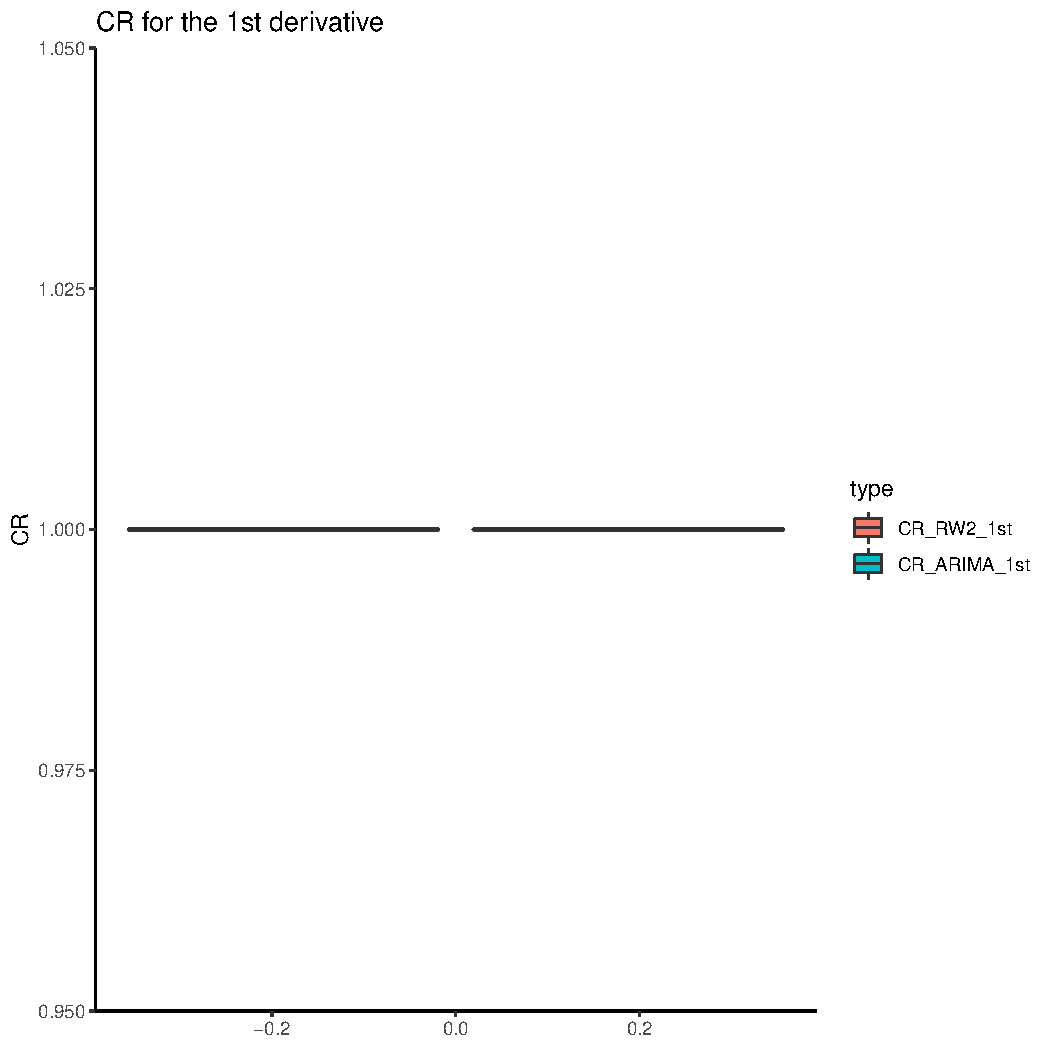
\includegraphics[width=0.29\textwidth]{sim2-g1st-CR.pdf}
    }
         \subfigure[rIAE for $g''$]{
      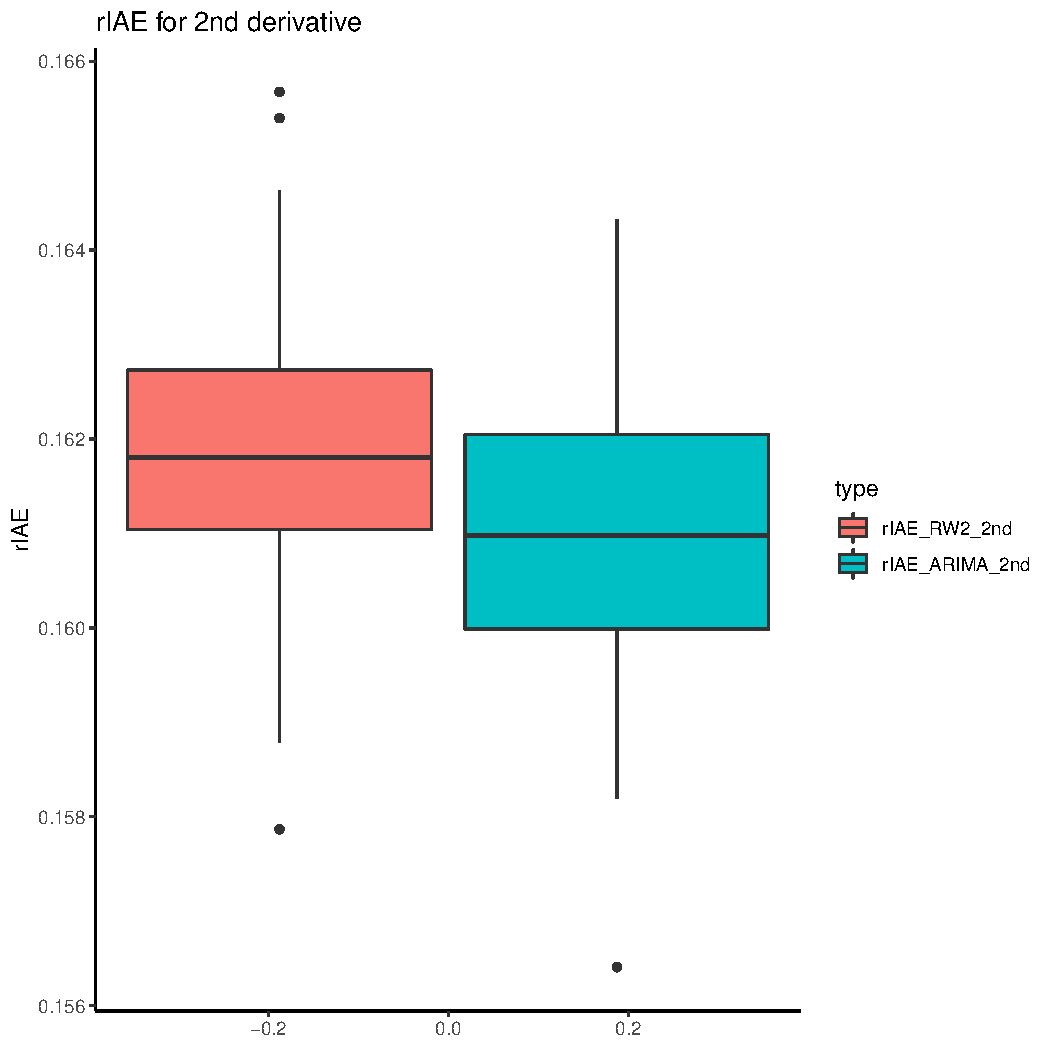
\includegraphics[width=0.29\textwidth]{sim2-g2nd-rIAE.pdf}
    }
        \subfigure[MCI for $g''$]{
      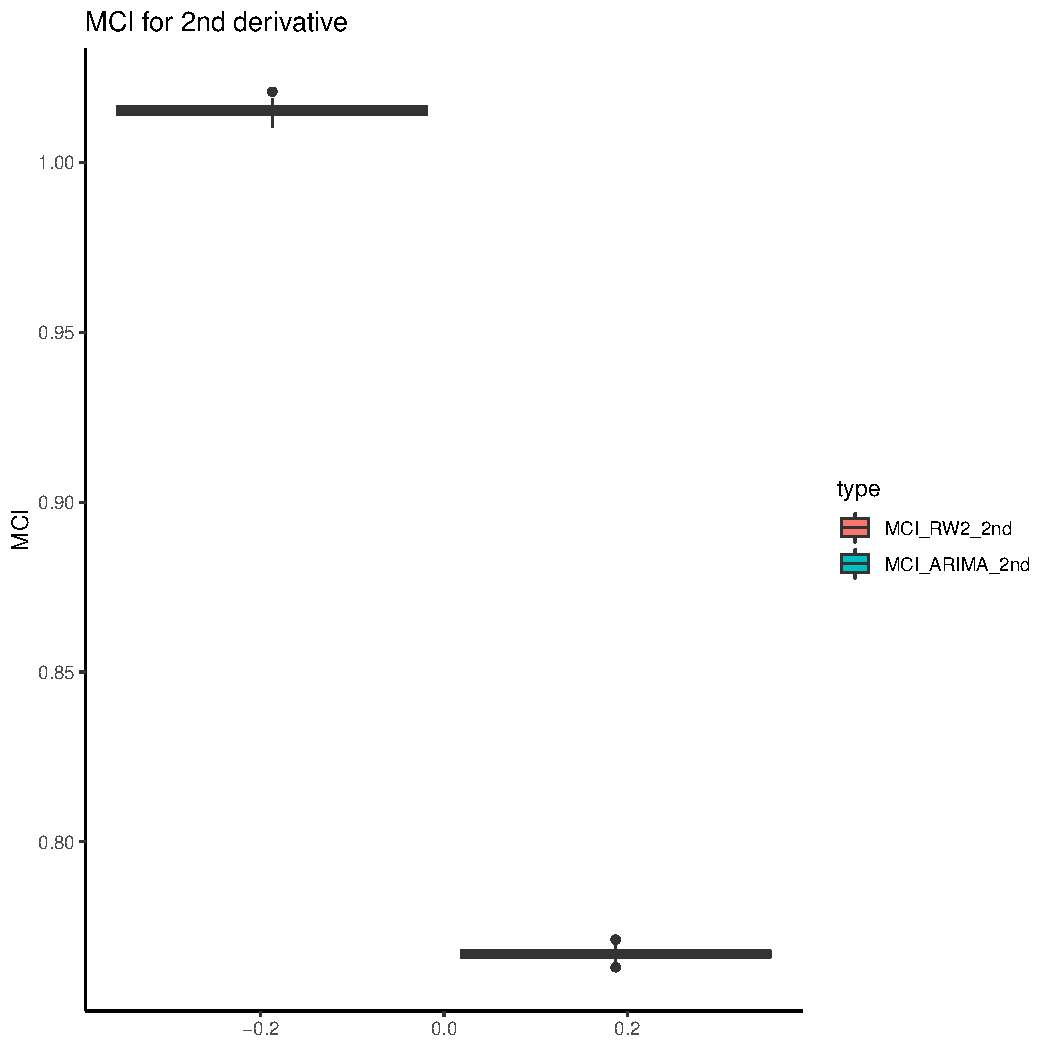
\includegraphics[width=0.29\textwidth]{sim2-g2nd-MCI.pdf}
    }
     \subfigure[CR for $g''$]{
      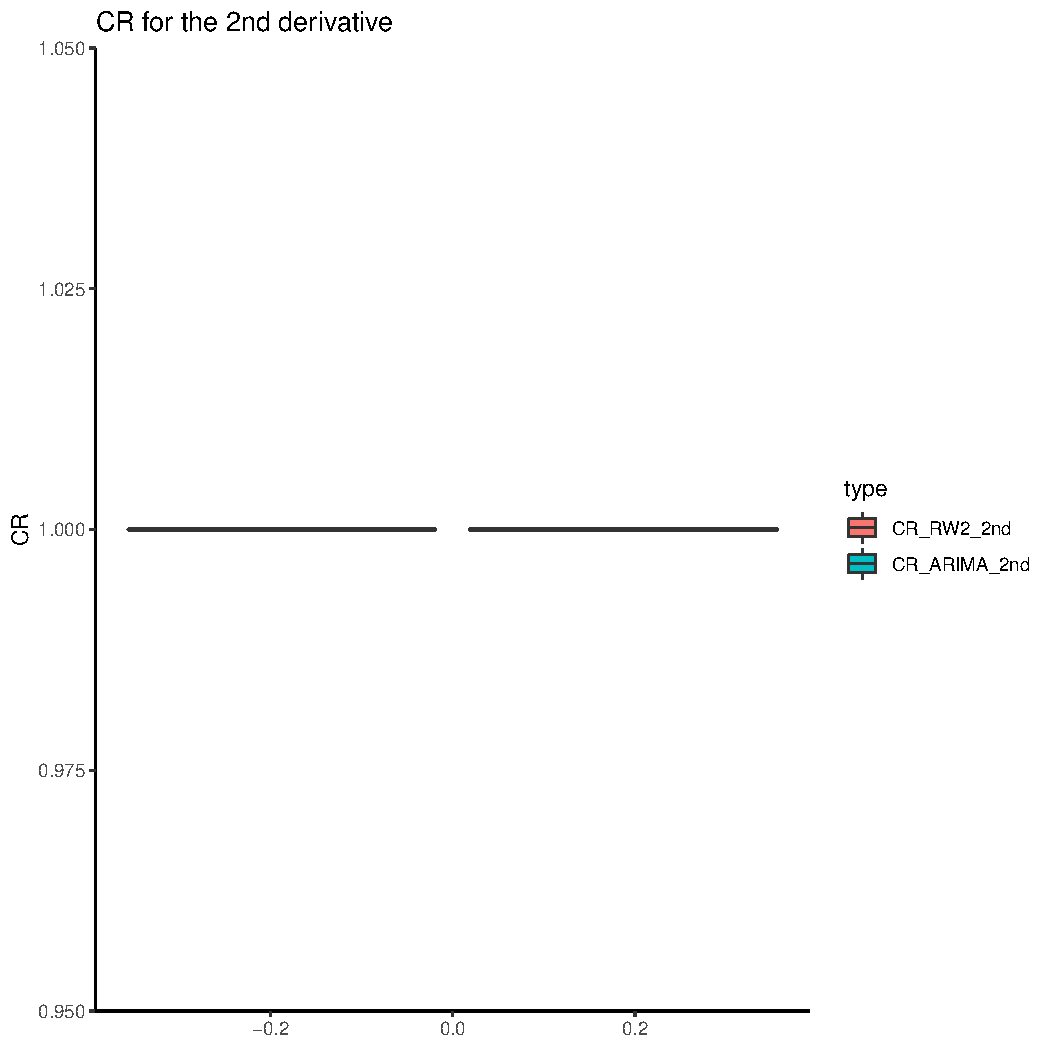
\includegraphics[width=0.29\textwidth]{sim2-g2nd-CR.pdf}
    }
    \caption{Inference for $g,g',g''$ using different methods for simulation 2, being replicated for 100 independent data sets.}
    \label{fig:sim2-100replic}
\end{figure}




\end{document}